% !TeX spellcheck = cs_CZ
% Basis of Linear Algebra:
%{\tikzset{external/prefix={tikz/MAI/}}
% \tikzset{external/figure name/.add={ch02_}{}}
%---------------------------------------------------------------------------------------------------
% mai1ch02.tex
%---------------------------------------------------------------------------------------------------
% ==================================================================================================
% In linear algebra, a basis is a set of linearly independent vectors that, in a
% linear combination, can represent every vector in a given vector space or free
% module, or, more simply put, which define a "coordinate system".[1] In more
% general terms, a basis is a linearly independent spanning set. 
% --------------------------------------------------------------------------------------------------
\setchaptertoc
\chapter{Všemocná úměra aneb lineární algebra poprvé}\label{mai:IchapII}

  Tuto kapitolu bychom mohli opatřit podtitulem \emph{„To nejnutnější z lineární algebry“}. Dovíme
  se v ní, co je třeba si představit pod pojmem \emph{„linearita“}, najdeme příklady linearity v
  geometrii i v přírodovědě (fyzice, chemii, biologii) a formulujeme základní poznatky týkající se
  řešení soustav lineárních rovnic. Do této oblasti patří i počítání s vektory a maticemi - objekty,
  které jsou velmi vhodné k vyjádření fyzikálních veličin.
    
  \section{Lineární rovnice}\label{mai:IchapIIsecI}
    Co tedy znamená slovo \textbf{linearita}? Pochází z latiny, \emph{linea recta = přímka}, 
    česky bychom řekli \emph{přímá úměrnost} nebo jen jednoduše \emph{úměra}.
    
    Nejjednodušší příklady linearity patří do oblasti geometrie - vyjádření \emph{přímek} a 
    \emph{rovin}. Jistě si ze střední školy vzpomínáme, že body těchto útvarů popisujeme jejich 
    souřadnicemi na přímce \(\mathbb{R}\), v rovině \(\mathbb{R}^2\), v prostoru \(\mathbb{R}^3\). 
    Souřadnice bodu v rovině tedy tvoří \emph{uspořádanou dvojici} reálných čísel, v prostoru pak 
    \emph{uspořádanou trojici} reálných čísel. (Pozor, dvojice \([a, b]\) a \([b, a]\) představují 
    různé body.)
    
    %--Parametrické vyjádření přímky--------------------------------
        % !TeX spellcheck = cs_CZ
% Musilova2009MA1
\wikitextrule
\begin{example}\label{mai:exam001}
  \textbf{Parametrické vyjádření přímky}\newline\small
  \emph{Přímka} — jednorozměrný lineární útvar v jednorozměrném prostoru \(\mathbb{R}^1\), 
  dvojrozměrném prostoru \(\mathbb{R}^2\), trojrozměrném prostoru \(\mathbb{R}^3\) (nebo i 
  n-rozměrném prostoru \(\mathbb{R}^n\)), je určena dvěma body, třeba \(A\) a \(B\), nebo 
  ekvivalentně, bodem \(A\) a \emph{směrovým} vektorem \(\vec{u}\) (obr. \ref{mai:fig000}). 
  Je-li \(X\) obecným bodem na této přímce, je vektor \(\overrightarrow{AX}\) rovnoběžný, 
  tj. \emph{kolineární}, se směrovým vektorem \(\vec{u}\). (Jako směrový můžeme samozřejmě 
  použít i vektor \(\overrightarrow{AB}\).) Vektor \(\overrightarrow{AX}\) má tedy s 
  vektorem \(\vec{u}\) stejný směr, lišit se může velikostí nebo orientací. Tuto skutečnost 
  zapíšeme tak, že \(\overrightarrow{AX}\) je \(t\)-násobkem vektorů \(\vec{u}\),
  \begin{equation*}
  \overrightarrow{AX} = t \cdot \vec{u}.
  \end{equation*}
  {\centering
    \captionsetup{type=figure}
    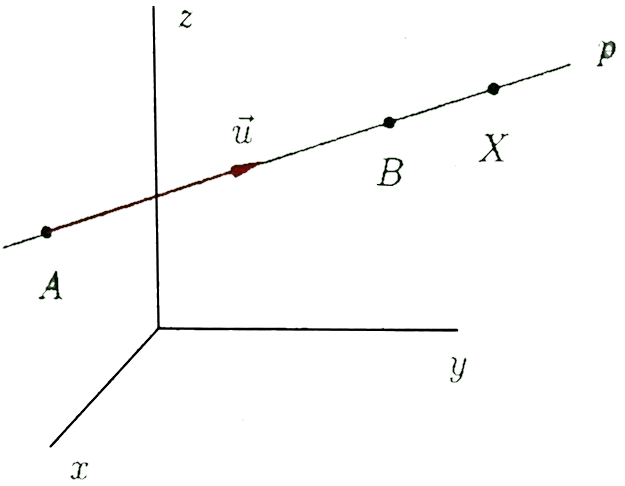
\includegraphics[width=0.4\linewidth]{mai_fig000.png}
    \captionof{figure}{Zadáni přímky. \cite[s.~1]{Musilova2009MA1}
    \label{mai:fig000}}
    \par}
  Veličinou \(t\), takzvaným \emph{parametrem}, který může nabývat všech reálných hodnot, 
  \(t\in\mathbb{R}\), dokážeme popsat všechny vektory \(\overrightarrow{AX}\), jejichž 
  koncový bod \(X\) leží na přímce \(p\). Naopak, žádné jiné body \(X\) než ty, které leží na 
  přímce \(p\), tuto vlastnost nemají. S označením bodů \(A\), \(X\), resp. vektorů 
  \(\vec{u}\), \(\overrightarrow{AX}\) kartézskými souřadnicemi, resp. složkami
  \begin{align*}
                    A &= (x_A,y_A, z_A), \\ 
                    X &=(x,y,z),         \\
              \vec{u} &= (u_1,u_2,u_3),  \\ 
  \overrightarrow{AX} &= (x - x_A, y - y_1A, z-z_A),
  \end{align*}
  dostáváme \textbf{parametrické vyjádřeni přímky} \(p\) ve tvaru
  \begin{equation}\label{MAI:eq_M001}
    p = \left\{(x,y,z)\in\mathbb{R}^3\,|\,
    \begin{matrix}
      x = x_A + tu_1,        \\
      y = y_A + tu_2,        \\
     z = z_A + tu_3,
    \end{matrix}
    \;t\in\mathbb{R}
    \right\}. 
  \end{equation}
  \normalsize
\end{example}
    %---------------------------------------------------------------

    Vidíme, že kartézské souřadnice bodu na přímce se vůči souřadnicím bodu \(A\) mění přímo 
    úměrně v závislosti na hodnotě parametru \(t\), tj. závisí na jeho první mocnině. Příslušná 
    závislost se nazývá \textbf{lineární funkcí}.

    Obdobně zapíšeme parametrické vyjádření roviny v \(\mathbb{R}^3\):
    
    %--Parametrická vyjádření roviny--------------------------------
    % !TeX spellcheck = cs_CZ
\begin{mathexam}{Parametrická vyjádření roviny}{exam004}
  Rovina v trojrozměrném prostoru \(\mathbb{R}^3\) je zadána třemi body \(A\), \(B\) a \(C\), které
  nesmějí ležet v jedné přímce, popřípadě dvěma body \(A\) a \(B\) a vektorem \(\vec{v}\)
  nerovnoběžným s \(\overrightarrow{AB}\), anebo bodem \(A\) a dvěma nerovnoběžnými směrovými
  vektory \(\vec{u}\) a \(\vec{v}\) (obr. \ref{mai:FIG002}). Všechny tyto typy zadání jsou
  ekvivalentní. Lze volit například \(\vec{u} = \overrightarrow{AB}\), \(\vec{v} =
  \overrightarrow{AC}\). Je-li \(X\) libovolným bodem roviny \(\varrho\), jsou vektory
  \(\overrightarrow{AX}\), \(\vec{u}\) a \(\vec{v}\) \textbf{lineárně závislé}. To znamená, že
  existují taková reálná čísla \(r\) a \(s\), že vektor \(\overrightarrow{AX}\) lze zapsat jako
  lineární kombinaci

  \begin{equation*}
    \overrightarrow{AX} = r\cdot\vec{u} + s\cdot\vec{v}, \qquad r,s \in\mathbb{R}
  \end{equation*}
  Při obdobném zápisu kartézských souřadnic bodů a složek vektorů jako u vyjádření přímky dostaneme
  parametrické vyjádření roviny \(\varrho\)
  \begin{equation*}
    \varrho = \left\{
    \begin{matrix}  
      (x,y,z)\in\mathbb{R}^3  \\
      r, s \in\mathbb{R}
    \end{matrix}
    \,\left\lvert\,
    \begin{matrix}
      x = x_A + ru_1 + sv_1,        \\
      y = y_A + ru_2 + sv_2,        \\
      z = z_A + ru_3 + sv_3,
    \end{matrix}\right.          
    \right\}.
  \end{equation*} 

  { \centering
    \captionsetup{type=figure}
    \luafigure[1]{mai_fig026.pdf}
    \captionof{figure}{Zadání roviny. \cite[s.~3]{Musilova2009MA1}
    \label{mai:FIG002}} \par}

  Toto vyjádření obsahuje opět lineární závislost: Souřadnice \(x\), \(y\) a \(z\) se vůči
  souřadnicím bodu \(A\) mění v závislosti na prvních mocninách parametrů \(r\) a \(s\). Můžeme tak
  hovořit o jakési „vícerozměrné úměře“.
\end{mathexam}
  
    %---------------------------------------------------------------

    Všimněme si nyní příkladů linearity z oblasti přírodovědy.
    
    %--Fyzika - Ohmův zákon-----------------------------------------
    % !TeX spellcheck = cs_CZ
% \wikitextrule
\begin{mdframed}[style=mdexam]
  \begin{example}\label{mai:exam035}
    \textbf{Fyzika - Ohmův zákon:}\newline
    Z elektřiny víme, že některé vodiče či elektrické prvky se při průchodu elektrického proudu 
    chovají podle zákona linearity: Proud, který jimi protéká, závisí přímo úměrně na přiloženém 
    napětí (obr. \ref{mai:fig036}). Platí \(I(U) = R^{-1 }U\) s konstantou úměrnosti \(R^{-1}\), kde 
    \(R\) je elektrický odpor vodiče (prvku).

    Pozn. 1: Předpokládáme, že elektrický odpor voltmetru je tak velký, že proud jím procházející je 
    z hlediska přesnosti měření zanedbatelný.
    
    Pozn. 2: Graf závislosti proudu na napětí na obrázku \ref{mai:fig036} může pro vyšší hodnoty 
    napětí vykazovat odchylku od linearity (přímkové závislosti), neboť se prvek při vyšším proudu 
    zahřívá a jeho odpor roste.
    
    {\centering
      \captionsetup{type=figure}
      \luafigure[1]{mai_fig036.png}
      \captionof{figure}{Chování lineárního vodiče (Ohmův zákon). \cite[s.~15]{Musilova2009MA1}
      \label{mai:fig036}}
      \par}  
  \end{example}
\end{mdframed}
    %---------------------------------------------------------------

    %--Fyzika - speciální typy pohybů-------------------------------
    % !TeX spellcheck = cs_CZ
\wikitextrule
\begin{example}\label{mai:exam036}
  \textbf{Fyzika — speciální typy pohybů:}\newline\small
  Při rovnoměrném pohybu tělesa (ať již přímočarém či křivočarém) je dráha, kterou těleso urazí za 
  dobu \(t\), přímo úměrná velikosti jeho rychlosti \(v\), tj. \(s(t) = s_0 + vt\). Při pohybu 
  rovnoměrně zrychleném (zpožděném) je lineární závislost velikosti rychlosti na čase, tj. \(v(t) = 
  v_0 \pm at\) při pohybu přímočarém (\(a\) je velikost zrychlení), nebo \(v(t) = v_0 \pm a_\tau 
  t\) při pohybu křivočarém (\(a_\tau\) je velikost průmětu zrychlení do směru tečny k 
  trajektorii tělesa — tečného zrychlení).
  \normalsize
\end{example}
    %---------------------------------------------------------------
    
    \subsection{Soustavy lineárních rovnic a jejich rychlé řešení}\label{mai:IchapIIsecIssecI}
      Příkladů linearity v přírodě bychom mohli nalézt bezpočet. Vraťme se však k matematice a k
      problematice uvedené v názvu tohoto odstavce, k soustavám lineárních rovnic. Začněme
      jednoduchou slovní úlohou ze základní školy:
      
      %--Jeníček a Mařenka kradli ježibabě perník---------------------
      % !TeX spellcheck = cs_CZ
% \wikitextrule
\begin{mdframed}[style=mdexam]
  \begin{example}\label{mai:exam037}
    \textbf{Jeníček a Mařenka kradli ježibabě perník:}\newline
    Dohromady snědli \num{11} perníkových srdíček. Jeníček jich přitom zkonzumoval o \num{3} více
    než Mařenka. Otázka je tradiční - kolik srdíček snědl každý z nich? Označíme-li \(M\) počet
    kousků, které snědla Mařenka a \(J\) počet srdíček, na nichž si pochutnal Jenda, můžeme
    informace zadané v úloze zapsat takto:
    \begin{equation*}
      M + J = 11, \qquad J = M + 3.
    \end{equation*}
    
    Řešení není problémem, snadno vidíme, že \(M = 4\) a \(J = 7\).
  \end{example}
\end{mdframed}
      %---------------------------------------------------------------
      
      O samotné řešení této jednoduché úlohy v tuto chvíli nejde. Pojmenujme si však vztahy, které
      jsme pro neznámé hodnoty \(M\) a \(J\) ze zadání úlohy dostali. Neznámé vystupují v rovnicích
      v první mocnině, tedy \emph{lineárně}. Máme \emph{soustavu dvou rovnic} o dvou neznámých \(M\)
      a \(J\). Úvahu snadno zobecníme: Předpokládejme, že máme neznámé veličiny
      \begin{equation*}
        (x_1, x_2, \ldots, x_n)
      \end{equation*}
      a máme o nich \(m\) informací, které lze zapsat ve tvaru lineárních rovnic (neznámé budou v
      těchto rovnicích vystupovat v první mocnině),
      \begin{align}
        a_{11}x_1 + a_{12}x_2 + \ldots + a_{1n}x_n &= b_1,     \nonumber           \\
        a_{21}x_1 + a_{22}x_2 + \ldots + a_{2n}x_n &= b_2,     \label{mai:eq002}   \\
        .......................................... &= \ldots   \nonumber           \\
        a_{m1}x_1 + a_{m2}x_2 + \ldots + a_{mn}x_n &= b_m,     \nonumber
      \end{align}
      Soustavu (\ref{mai:eq002}) \textbf{nazýváme soustavou \(\mathbf{m}\) lineárních rovnic o
      \(\mathbf{n}\) neznámých}. Označme ji jako \(S\) a pod tímto označením se k ní budeme vracet.
      Soubory reálných čísel \((a_{ij})\) a \((b_i)\), kde \(1 \leq i \leq m\), \(1 \leq j \leq n\),
      jsou zadány. Lze je uspořádat do takzvaných \textbf{matic}:
      \begingroup
        \renewcommand\arraycolsep{3pt}
        \begin{equation*}
          \matr{A} =
            \begin{pmatrix}[0.9]
              a_{11} & a_{12} & \ldots & a_{1n} \\
              a_{21} & a_{22} & \ldots & a_{2n} \\
              \ldots & \ldots & \ldots & \ldots \\
              a_{m1} & a_{m2} & \ldots & a_{mn}          
            \end{pmatrix},\quad
            \overline{\matr{B}} =
            \begin{pmatrix}[0.9]
              b_1     \\
              b_2     \\
              \ldots  \\
              b_m 
            \end{pmatrix}
        \end{equation*}
      \endgroup

      Matice \(\matr{A}\) je typu \(m/n\), má \(m\) řádků a \(n\) sloupců, \(i\) je řádkový index a
      \(j\) je sloupcový index. Matice \(\overline{\matr{B}}\) je typu \(m/1\) (\(m\) řádků a jeden
      sloupec), hovoříme také o sloupcové matici. Soustavu \(S\) můžeme zapsat zkráceně pomocí
      maticového násobení (podrobněji viz později odstavec \ref{mai:IchapIIsecIII}):
      \begin{align}\label{mai:eq004}
        \matr{A} \cdot \matr{X} &= \overline{\matr{B}}, \quad \text{nebo} \nonumber\\
        \setlength{\arraycolsep}{3pt}
          \begin{pmatrix}[0.9]
            a_{11} & a_{12} & \ldots & a_{1n} \\
            a_{21} & a_{22} & \ldots & a_{2n} \\
            \ldots & \ldots & \ldots & \ldots \\
            a_{m1} & a_{m2} & \ldots & a_{mn}
          \end{pmatrix} \cdot
          \begin{pmatrix}[0.9]
            x_1     \\
            x_2     \\
            \ldots  \\
            x_m 
          \end{pmatrix}  &=
          \begin{pmatrix}[0.9]
            b_1     \\
            b_2     \\
            \ldots  \\
            b_m 
          \end{pmatrix}
      \end{align} 
      V tuto chvíli vysvětlíme podstatu maticového násobení jen technicky: Násobit mezi sebou
      můžeme matici \(\matr{A} = (a_{ij})\) typu \(m/n\) (levý činitel) a matici \(\matr{C} =
      (c_{jk})\) typu \(n/p\) (pravý činitel, činitele nelze zaměňovat). Výsledkem je matice
      \(\matr{D} = (d_{ik})\) typu \(m/p\), jejíž prvky se počítají podle předpisu
      \begin{equation}\label{mai:eq005}
        d_{ik} = \sum_{j=1}^{n} a_{ij}\cdot c_{jk}.
      \end{equation}
      
      Z tohoto obecného předpisu vidíme, že levé strany soustavy \(S\) lze interpretovat ve tvaru
      součinu matice \(A\) typu \(m/n\) s maticí neznámých typu \((n/1)\), výsledkem je matice
      pravých stran \(\overline{\matr{B}}\), která je typu \(m/1\). Matice \(\matr{A}\) se nazývá
      \textbf{maticí soustavy}. Matice, která vznikne jejím \emph{rozšířením} o sloupec pravých
      stran, tj.
      \begingroup
        \renewcommand\arraystretch{0.8}
        \renewcommand\arraycolsep{3pt}
        \begin{equation*}
          \matr{B} = (\matr{A}\lvert\overline{\matr{B}}) =
          \left(
            \begin{array}{cccc|c}
              a_{11} & a_{12} & \ldots & a_{1n} & b_1    \\
              a_{21} & a_{22} & \ldots & a_{2n} & b_2    \\
              \ldots & \ldots & \ldots & \ldots & \ldots \\
              a_{m1} & a_{m2} & \ldots & a_{mn} & b_m 
            \end{array}
          \right)
        \end{equation*}
      \endgroup
      je pak \textbf{rozšířenou maticí soustavy}. Je-li sloupec pravých stran soustavy tvořen samými
      nulami, nazývá se soustava \textbf{homogenní}, v opačném případě \textbf{nehomogenní}. Řešením
      soustavy \(S\) nazýváme každou \(n\)-tici \((x_i, x_2,\ldots, x_n)\), která soustavu \(S\)
      splňuje. Cílem je najít všechna řešení soustavy \(S\). Abychom řešení nalezli, musíme soustavu
      upravovat, zjednodušovat. Prováděné úpravy mají vést k jednodušší, avšak ekvivalentní soustavě
      rovnic, tj. takové, která má naprosto stejný soubor všech řešení jako soustava původní. Takové
      úpravy nazýváme \textbf{ekvivalentními}. Dvě základní, pomocí nichž lze uskutečnit všechny
      ostatní, jsou
      \begin{mdframed}[style=highlight]
        \begin{itemize}[noitemsep]
          \item vynásobení libovolné, například \(i\)-té, rovnice libovolným \emph{nenulovým}
                číslem,
          \item přičtení \(i\)-té rovnice vynásobené libovolným číslem k \(l\)-té rovnici.
        \end{itemize} 
      \end{mdframed}
      V soustavě lze samozřejmě také měnit pořadí rovnic. Tato úprava je rovněž ekvivalentní.
      Nevypisujeme ji však zvlášť proto, že ji lze realizovat pomocí vhodně zvolené posloupnosti
      základních dvou úprav.
      
      Abychom nemuseli soustavu stále opisovat i s neznámými, provádíme obvykle ekvivalentní úpravy
      jen s maticí \(\matr{B} = (\matr{A}\vert\overline{\matr{B}})\) (každý řádek této matice
      představuje jednu rovnici soustavy \(S\)). Může se stát, že soustava má právě \emph{jedno
      řešení}, jako tomu bylo v  úloze o Mařence a Jeníčkovi. Také nemusí mít \emph{řešení žádné},
      jako například soustava \(x + y = 0\), \(x + y = 1\) (součet dvou čísel nemůže nabývat
      současně dvou různých hodnot). A třeba má také řešení \emph{nekonečně mnoho} (řešením soustavy
      jedné rovnice o dvou neznámých \(x + y = 1\) jsou všechny dvojice tvaru \((x, 1 - x)\), kde
      \(x\) je libovolné). A může mít soustava \(S\) třeba právě dvě řešení? Prostřednictvím
      následujícího příkladu ukážeme metodu, která vede velmi rychle k nalezení všech řešení a
      umožňuje také vyslovit obecné závěry o jejich vlastnostech a počtu. Jedná se o
      \textbf{Gaussovu eliminační metodu}.

      %Gaussova eliminační metoda-------------------------------------
      \begin{mathexam}{Gaussova eliminační metoda}{exam038}
  Je zadána soustava tří (\(m = 3\)) rovnic o pěti (\(n = 5\)) neznámých:
  \begin{alignat*}{7}
       x_1 &+ 2x_2 &-  x_3 &+  x_4 &- 5x_5 &=  &&0, \\
     -2x_1 &- 4x_2 &+ 2x_3 &+ 4x_4 &+ 4x_5 &= -&&6, \\
      -x_1 &- 2x_2 &+  x_3 &+ 5x_4 &-  x_5 &=  &&6.
  \end{alignat*}
  Budeme provádět ekvivalentní úpravy matice \(\matr{B}\) tak, abychom ji zjednodušovali.
  Ekvivalenci matic budeme označovat znakem \(\sim\). 
  \begingroup
    \renewcommand\arraystretch{1.0}
    \renewcommand\arraycolsep{3pt}
    \begin{equation*}
      \matr{B} = (\matr{A}\lvert\overline{\matr{B}}) =
      \left(
        \begin{array}{rrrrr|r}
           1 &  2 & -1 & 1 & -5 &  0    \\
          -2 & -4 &  2 & 4 &  4 & -6    \\
          -1 & -2 &  1 & 5 & -1 &  6
        \end{array}
      \right).
    \end{equation*}
  \endgroup
  V prvním řádku je na první pozici jednička. Toho využijeme k snadné „likvidaci“, tedy eliminaci,
  prvních prvků v druhém a třetím řádku pomocí elementárních úprav. Provedeme tyto dvě úpravy:
  první řádek vynásobený číslem \num{2} přičteme k druhému řádku, první řádek přičteme ke třetímu
  řádku. Dostaneme
  \begingroup
    \renewcommand\arraystretch{1.0}
    \renewcommand\arraycolsep{3pt}
    \begin{equation*}
      \matr{B} \sim
      \left(
        \begin{array}{rrrrr|r}
          1 &  2 & -1 & 1 & -5 &  0         \\
          \bm{0} &  0 &  0 & 6 & -6 & -6    \\
          \bm{0} &  0 &  0 & 6 & -6 &  6
        \end{array}
      \right).
    \end{equation*}
  \endgroup  
  Vidíme, že jsme v druhém i třetím řádku dostali na první sloupcové pozici nulu (tučná). (Nuly na
  dalších  pozicích vznikly náhodou, vlivem jednoduchosti zadání.) Nyní vynásobíme druhý i třetí
  řádek číslem (\num{1/6}):
  \begingroup
    \renewcommand\arraystretch{1.0}
    \renewcommand\arraycolsep{3pt}    
    \begin{equation*}
      \matr{B} \sim
      \left(
        \begin{array}{rrrrr|r}
                1 &  2 & -1 & 1 & -5 &  0    \\
                0 &  0 &  0 & 1 & -1 & -1    \\
                0 &  0 &  0 & 1 & -1 &  1
        \end{array}
      \right).
    \end{equation*}
  \endgroup  
  Přestože již nyní vidíme, že soustava nemá řešení (rovnice druhého a třetího řádku znějí \(x_4 -
  x_5 = - 1\) a \(x_4 -x_5 = 1\), takže jim nevyhovuje žádná dvojice čísel \((x_4, x_5)\)), budeme
  v eliminaci pokračovat. Další úpravy se již týkají pouze druhého a třetího řádku. Druhý řádek
  vynásobený (\num{-1}) přičteme ke třetímu. Pak

  \begingroup
  \renewcommand\arraystretch{1.0}
  \renewcommand\arraycolsep{3pt}
    \begin{equation*}
      \matr{B} \sim
      \left(
        \begin{array}{rrrrr|r}
                1 &  2 & -1 & 1      & -5 &  0    \\
                0 &  0 &  0 & 1      & -1 & -1    \\
                0 &  0 &  0 & \bm{0} &  0 &  2
        \end{array}
      \right).
    \end{equation*}
  \endgroup  
  Získáváme tak ekvivalentní soustavu rovnic
  \begin{alignat*}{5}
        x_1 + 2x_2 - x_3 &+  x_4 &- 5x_5 &=  &&0, \\
                         &+  x_4 &-  x_5 &= -&&1, \\
                         &       &     0 &=  &&2.
  \end{alignat*}
  V poslední rovnici je ihned vidět rozpor - soustava nemá řešení
\end{mathexam}
      %---------------------------------------------------------------

      Na základě výsledného tvaru matice soustavy a rozšířené matice soustavy získané ekvivalentními
      úpravami soustavy \(S\) nyní formulujeme obecné kritérium pro to, aby soustava S měla vůbec
      nějaké řešení. Matice \(\matr{A}\) i \(\matr{B}\) se po provedení ekvivalentních úprav dostaly
      do velmi jednoduchého tvaru, který připomíná schodiště obrácené „vzhůru nohama“, odmyslíme-li
      si nuly v levé části jednotlivých řádků (následující zápis pouze usnadňuje názornou představu,
      znak ekvivalence již psát nemůžeme):
      \begingroup
        \renewcommand\arraystretch{0.9}
        \renewcommand\arraycolsep{3pt}
        \begin{align*}
          \matr{A} &\ldots
          \left(
            \begin{array}{rrrrr}
                    1 &  2 & -1 & 1      & -5     \\
                      &    &    & 1      & -1 
            \end{array}
          \right),  \\
          \matr{B} &\ldots
          \left(
            \begin{array}{rrrrr|r}
                    1 &  2 & -1 & 1      & -5 &  0    \\
                      &    &    & 1      & -1 & -1
            \end{array}
          \right).
        \end{align*}
      \endgroup

      Všimněme si, že „schodiště“ jsou nepravidelná, pokud jde o šířku schodů, výška všech schodů je
      však stejná - jeden řádek. Tímto způsobem je dán \emph{schodovitý tvar} matice \(\matr{A}\),
      resp. \(\matr{B}\). Úzce s ním souvisí důležitá charakteristika matice, která je nezávislá jak
      na provedených úpravách tak na výsledném schodovitém tvaru. Je to hodnost matice, definovaná
      takto:      
      \begin{mdframed}[style=highlight] 
        \textbf{Hodnost} matice je počet nenulových řádků jejího schodovitého tvaru.
      \end{mdframed}
      V našem příkladu je hodnost matice \(\matr{A}\) soustavy \(S\) rovna dvěma, hodnost matice
      rozšířené \(\matr{B}\) je rovna třem. Píšeme
      \begin{equation*}
        h(\matr{A}) = 2,\qquad h(\matr{B}) = 3.
      \end{equation*}
      
      \begin{mdframed}[style=mdnote] 
        \begin{note}
          Že lze získat schodovitý tvar různými posloupnostmi ekvivalentních úprav je zřejmé. Uvědomme
          si však, že ani výsledný schodovitý tvar není určen jednoznačně - stačí třeba vynásobit
          některý řádek dvěma a výsledná matice ekvivalentní s původní je rovněž schodovitá. Poněvadž
          má matice \(\matr{B}\) o jeden sloupec více než matice \(\matr{A}\), platí vždy
          \(h(\matr{A}) < h(\matr{B})\). V případě \(h(\matr{A}) < h(\matr{B})\) pak \(h(\matr{A}) =
          h(\matr{B}) - 1\). Jak názorně ukazuje náš příklad, má pro \(h(\matr{A}) < h(\matr{B})\)
          některá z rovnic ekvivalentní soustavy tvar \(0 = 1\), soustava tedy nemá řešení. Můžeme tak
          formulovat kritérium (podmínku nutnou a postačující) řešitelnosti soustavy lineárních
          rovnic.
        \end{note}
      \end{mdframed}
      
      \begin{lemma}\label{mai:lemma001}
        (\textbf{Frobeniova}): Soustava lineárních rovnic má řešení právě tehdy, je-li hodnost její
        matice rovna hodnosti matice rozšířené.
      \end{lemma}
      
      Ihned vidíme, že homogenní soustava má podle této věty řešení vždy, neboť poslední sloupec
      její rozšířené matice je složen ze samých nul. Skutečně, jedním ze souboru řešení každé
      homogenní soustavy je \(n\)-tice
      \begin{equation*}
        (x_1, x_2, \ldots, x_n) = (0, 0, \ldots, 0),
      \end{equation*}
      zvaná \textbf{triviální řešení}.
      
      Nyní se vraťme k otázce, jak zjistit, kolik řešení má daná soustava, a jak je všechna popsat.
      Poslouží nám příklad \ref{mai:exam038} v mírné obměně spočívající v záměně koeficientu \(b_3\)
      z hodnoty \num{6} na \num{-6}.
      
      %Ještě jednou Gaussova eliminační metoda------------------------
      % !TeX spellcheck = cs_CZ
\wikitextrule
\begin{example}\label{mai:exam039}
  \textbf{Ještě jednou Gaussova eliminační metoda}\newline\small
  Je zadána soustava rovnic:
  \begin{alignat*}{7}
      x_1 &+ 2x_2 &-  x_3 &+  x_4 &- 5x_5 &=  &&0, \\
    -2x_1 &- 4x_2 &+ 2x_3 &+ 4x_4 &+ 4x_5 &= -&&6, \\
     -x_1 &- 2x_2 &+  x_3 &+ 5x_4 &-  x_5 &= -&&6.
  \end{alignat*}
  Rozšířená matice soustavy má nyní tvar 
  \begin{equation*}
    \matr{B} = (\matr{A}|\overline{\matr{B}}) =
    \left(
      \begin{array}{rrrrr|r}
         1 &  2 & -1 & 1 & -5 &  0    \\
        -2 & -4 &  2 & 4 &  4 & -6    \\
        -1 & -2 &  1 & 5 & -1 & -6
      \end{array}
    \right).
  \end{equation*}
  Stejné ekvivalentní úpravy jako v příkladu \ref{mai:exam038} vedou nyní k výsledku
  \footnotesize %\small \scriptsize \tiny
  \begin{equation*}
    \matr{B} \sim
    \left(
      \begin{array}{rrrrr|r}
         1 &  2 & -1 & 1 & -5 &  0         \\
         \bm{0} &  0 &  0 & 6 & -6 & -6    \\
         \bm{0} &  0 &  0 & 6 & -6 & -6
      \end{array}
    \right) \sim
    \left(
      \begin{array}{rrrrr|r}
              1 &  2 & -1 & 1 & -5 &  0    \\
              0 &  0 &  0 & 1 & -1 & -1    \\
              0 &  0 &  0 & 1 & -1 & -1
      \end{array}
    \right) \sim
    \left(
      \begin{array}{rrrrr|r}
              1 &  2 & -1 & 1      & -5 &  0    \\
              0 &  0 &  0 & 1      & -1 & -1    \\
              0 &  0 &  0 & \bm{0} &  0 &  0
      \end{array}
    \right).
  \end{equation*}\normalsize
  Nyní platí \(h(\matr{A}) = h(\matr{B}) = 2\). Podle Frobeniovy věty \ref{mai:lemma001} tedy 
  soustava určitě má řešení. Ekvivalentní soustava má tvar
  \begin{alignat*}{5}
         x_1 + 2x_2 - x_3 &+  x_4 &- 5x_5 &=  &&0, \\
                          &+  x_4 &-  x_5 &= -&&1, \\
                          &       &     0 &=  &&0.
  \end{alignat*}
  Poslední rovnice je identitou a můžeme ji vypustit. Máme pět neznámých a jen dvě nezávislé 
  rovnice. Dvě z neznámých tedy můžeme vyjádřit pomocí zbývajících. Postupujeme „odzadu“ , začínáme 
  druhou, jednodušší, rovnicí:
  \begin{align*}
                                                x_4 &= -1 + x_5,                \\
    x_1 = - 2x_2 + x_3 - x_4 + 5x_5 \Rightarrow x_1 &= -2x_2 + x_3 + 4x_5 + 1.
  \end{align*}
  Za neznámé vystupující na pravé straně, tj. \(x_2\), \(x_3\) a \(x_5\), můžeme dosazovat cokoli a 
  vždycky se k nějakým hodnotám \(x_1\) a \(x_4\) dopočítáme. Všechna řešení soustavy \(S\) proto 
  můžeme zapsat v obecném tvaru
  \begin{equation}\label{mai:eq040}
    (-2x_2 + x_3 + 4x_5 + 1, x_2, x_3, x_5 - 1, x_5).
  \end{equation}
  \normalsize
\end{example}
      %---------------------------------------------------------------
      
      Soubor řešení ve tvaru (\ref{mai:eq040}) se nazývá obecným řešením soustavy. Jeho jednotlivé
      prvky, jednotlivá konkrétní řešení soustavy, jsou dány volbou volných neznámých \(x_2\),
      \(x_3\) a \(x_5\). Také z příkladu \ref{mai:exam039} lze učinit obecný závěr:
      
      \begin{lemma}\label{mai:lemma002}
        Nechť pro soustavu \(m\) lineárních rovnic o \(n\) neznámých platí \(h(\matr{A}) =
        h(\matr{B}) = h\). Pak její obecné řešení závisí (lineárně) na \(d = n - h\) volných
        neznámých.
      \end{lemma}
      
      Číslo \(d\) se nazývá \textbf{dimenze prostoru řešení soustavy}. Tento pojem ještě podrobněji
      vysvětlíme později.
      
      Nyní již snadno zodpovíme otázku, čím je dána \emph{mohutnost souboru řešení soustavy
      lineárních rovnic}, tj. kolik má taková soustava řešení. Možnosti jsou pouze:
      \begin{mdframed}[style=highlight]
        \begin{itemize}[leftmargin=3pt,noitemsep]
          \item žádné řešení - pro \(h(\matr{A}) \neq h(\matr{B})\),
          \item právě jedno řešení - pro \(h = h(\matr{A}) = h(\matr{B})\) a současně \(h = n\),
                takže nezbývá žádná volná neznámá,
          \item nekonečně mnoho řešení - pro \(h = h(\matr{A}) = h(\matr{B})\) a současně \(h < n\),
                kdy máme k dispozici \(d = n - h\) volných neznámých.
        \end{itemize}  
      \end{mdframed}  
      Že by tedy třeba měla soustava právě dvě, tři či osmnáct řešení není možné.
      
      Jakési zvláštní postavení můžeme přisoudit \emph{homogenním soustavám}. Ty mají, jak jsme se
      již přesvědčili, řešení vždy, alespoň to triviální, složené ze samých nul. Zajímejme se o
      situaci, kdy má homogenní soustava i jiná, netriviální, řešení. U homogenní soustavy je
      hodnost její matice vždy shodná s hodností matice rozšířené, \(h = h(\matr{A}) =
      h(\matr{B})\). Je-li navíc \(h = n\), má podle obecného tvrzení \ref{mai:lemma002} soustava
      právě jedno řešení, jímž nutně je řešení triviální. V opačném případě, tj. pro \(h < n\), máme
      opět k dispozici \(d = n - h\) volných neznámých, a tedy nekonečně mnoho netriviálních řešení.
      Všimněme si ještě jedné zajímavosti u homogenní soustavy. Jsou-li dvě \(n\)-tice čísel \(X =
      (x_1, x_2, \ldots, x_n)\) a \(\overline{X} = (\overline{x}_1, \overline{x}_2, \ldots,
      \overline{x}_n)\) jejím řešením, pak také \(n\)-tice vytvořená jako jejich lineární kombinace
      \begin{equation*}
        \alpha\cdot X + \overline{\alpha}\cdot\overline{X} = 
          (\alpha x_1, \alpha x_2, \ldots, \alpha x_n) + 
          (\overline{\alpha}\,\overline{x}_1, 
          \overline{\alpha}\,\overline{x}_2, \ldots, 
          \overline{\alpha}\,\overline{x}_n)
      \end{equation*}
      kde \(\alpha\) a \(\overline{\alpha}\) jsou libovolná čísla, je \emph{řešením soustavy}.
      Možnost tohoto „lineárního kombinování“ připadá samozřejmě v úvahu pro libovolný počet
      libovolných řešení soustavy. Fyzik by řekl, že soustava vyhovuje principu superpozice.
      Soustava nehomogenní tu to vlastnost nemá „vinou“ nenulového sloupce pravých stran.
    
    \subsection{Přímky a roviny - lineární geometrické útvary}
      Vraťme se ještě na chvíli k linearitě v geometrii a všimněme si problematiky vzájemné polohy
      přímek a rovin. Procvičíme si na ní mimo jiné i řešení soustav lineárních rovnic. V odstavci
      \ref{mai:IchapIIsecIssecI} jsme odvodili parametrické vyjádření přímky a roviny v
      trojrozměrném prostoru. Nyní se pokusíme z těchto vyjádření vyloučit parametry a získat obecné
      rovnice přímky a roviny, které již budou obsahovat pouze kartézské souřadnice bodů ležících v
      příslušné přímce či rovině. Začněme případem roviny.

      %--Obecná rovnice roviny----------------------------------------
      % !TeX spellcheck = cs_CZ
\wikitextrule
\begin{example}\label{mai:exam040}
  \textbf{Obecná rovnice roviny}\newline\small
  Parametrické rovnice roviny z příkladu \ref{mai:exam004} můžeme chápat jako soustavu tří rovnic o 
  dvou neznámých:
  \begin{align*}
      ru_1 + sv_1 &= x - x_A, \\
      ru_2 + sv_2 &= y - y_A, \\
      ru_3 + sv_3 &= z - z_A, 
  \end{align*}
  kde neznámými jsou parametry \(r\) a \(s\). Z geometrického významu této soustavy je zřejmé, že 
  pro každý bod \(X = (x, y, z)\), který leží v rovině \(\varrho\), bude soustava mít jako řešení 
  právě jednu dvojici parametrů \((r, s)\) (pro body, které v rovině neleží, soustava řešení nemá). 
  Vypočteme parametry \(r\) a \(s\) například z prvních dvou rovnic. Předpokládejme, že \(u_1 \neq 
  0\), a upravujme matici soustavy:
  
  \begin{equation*}
    \left(
      \begin{array}{rr|r}
         u_1 &  v_1  &  x-x_A         \\
         u_2 &  v_2  &  y-y_A
      \end{array}
    \right) \sim
    \left(
      \begin{array}{cc|c}
              u_1 &  v_1               & x - x_A     \\
              0   &  u_1v_2 - u_2v_1   & (y-y_A)u_1 - (x-x_A)u_2
      \end{array}
    \right).
  \end{equation*}
  odkud pro \((u_1v_2 — u_2v_1) \neq 0\) dostaneme
  \begin{equation*}
    r = - \dfrac{(y-y_A)v_1 - (x-x_A)v_2}{u_1v_2 - u_2v_1}, \qquad 
    s =   \dfrac{(y-y_A)u_1 - (x-x_A)u_2}{u_1v_2 - u_2v_1}
  \end{equation*}
  Dosadíme-li získané hodnoty do třetí rovnice (dá to trochu práce), dostáváme obecnou  rovnici roviny 
  \(\varrho\)
  \begin{subequations} % \label{mai:eq041}
    \begin{equation}\label{mai:eq041a}
      ax + by + cz + d= 0,
    \end{equation}
    \begin{equation}\label{mai:eq04b}
      a = u_2v_3 - u_3v_2, \qquad b = u_3v_1 - u_1v_3, \qquad c = u_1v_2 - u_2v_1,
    \end{equation}
    \begin{equation}\label{mai:eq041c}
      d = (u_2v_3 - u_3v_2)x_A - (u_3v_1 - u_1v_3)y_A - (u_1v_2 - u_2v_1)z_A.
    \end{equation}
  \end{subequations}
  Při tomto výpočtu vyvstaly některé problémy. Pokusme se je vyřešit:
  \begin{itemize}
    \item Aby získaná rovnice opravdu představovala nějakou rovinu, musí v ní zůstat alespoň jedna 
          ze souřadnic \(x, y, z\). Alespoň jedno z čísel \(a, b, c\) by tedy mělo být nenulové. 
          Dokažte, že tomu tak opravdu je, a využijte při tom skutečnosti, že vektory \(\vec{u}\) a 
          \(\vec{v}\) nesmí být rovnoběžné. Co znamená předpoklad \((u_1v_2 - u_2v_1) \neq 0\)?
    \item Předpokládali jsme, že \(u_1 \neq 0\). Jak budeme postupovat, nebude-li tento předpoklad  
          splněn? Lze v tomto případě použít obecné výrazy získané pro \(r\) a \(s\)?
  \end{itemize}
  \normalsize
\end{example}
      %---------------------------------------------------------------

      %--Obecná rovnice přímky----------------------------------------
      % !TeX spellcheck = cs_CZ
% \wikitextrule
\begin{mdframed}[style=mdexam]
  \begin{example}\label{mai:exam041}
    \textbf{Obecná rovnice přímky}\newline
    Přímku \(p\) si snadno představíme jako průsečnici dvou nerovnoběžných rovin \(\varrho\) a 
    \(\sigma\). Jejich rovnice tvoří soustavu, která představuje obecné rovnice přímky
      \begin{align*}
        \varrho &= \{(x, y, z)\in\mathbb{R}^3\mid a_1x+ b_1y+ c_1z+ d_1 = 0 \}  \\ 
        \sigma  &= \{(x, y, z)\in\mathbb{R}^3\mid a_2x+ b_2y+ c_2z+ d_2 = 0 \}, 
      \end{align*}
    Zkusme přijít na to, co musí platit pro koeficienty v rovnicích rovin, aby byly nerovnoběžné. 
    Jedna a táž přímka může být zadána různými dvojicemi nerovnoběžných rovin. Všechny roviny, které 
    přímkou \(p\) procházejí, tvoří geometrický útvar zvaný \textbf{svazek rovin prvního druhu}, 
    přímka sama je \textbf{osou} svazku. 
  \end{example}
\end{mdframed}
      %---------------------------------------------------------------
      
      %--Vektor rovnoběžný s rovinou----------------------------------
      % !TeX spellcheck = cs_CZ
\wikitextrule
\begin{example}\label{mai:exam042}
  \textbf{Vektor rovnoběžný s rovinou}\newline\small
   Ja k poznáme, zda je vektor \(\vec{u} = (u_1, u_2, u_3)\) rovnoběžný s rovinou \(ax + by + cz + 
   d = 0\)? Pokud vektor \(\vec{u}\) s rovinou rovnoběžný je, pak zcela jistě existují v této 
   rovině dva body \(A = (x_A, y_A, z_A)\) a \(B = (x_B, y_B, z_B)\) tak, že \(\overrightarrow{AB} 
   = \vec{u} = (x_B - x_A, y_B - y_A, z_B - z_A)\). Tyto body splňují rovnici roviny, tj.
   \begin{equation*}
     ax_A + by_A + cz_A + d = 0,\qquad ax_B + by_B + cz_B + d = 0.
   \end{equation*}
   Odečtením rovnic dostaneme kritérium rovnoběžnosti vektoru s rovinou \(au_1 + bu_2+ cu_3 = 0\).
   \normalsize
\end{example}
      %---------------------------------------------------------------
  
      Máme připraveno vše pro řešení otázky vzájemné polohy přímek a rovin.

      %--Vzájemná poloha tří rovin------------------------------------
      % !TeX spellcheck = cs_CZ
\wikitextrule
\begin{example}\label{mai:exam043}
  \textbf{Vzájemná poloha tří rovin}\newline\small
  Zapojme geometrickou představivost a uvažujme, jakou vzájemnou polohu mohou mít tři roviny
  \begin{align*}
    \varrho: a_1x + b_1y + c_1z + d_1 &= 0, \\
    \sigma : a_2x + b_2y + c_2z + d_2 &= 0, \\
    \tau   : a_3x + b_3y + c_3z + d_3 &= 0,
  \end{align*}
  Současně si uvědomme, že předchozí soustava je soustavou lineárních rovnic o neznámých \(x\), 
  \(y\) a \(z\), představujících souřadnice společných bodů rovin \(\varrho\), \(\sigma\) a 
  \(\tau\). Soustava je charakterizována maticí
  \begin{equation}\label{mai:eq043}
    \matr{B} = (\matr{A}|\overline{\matr{B}}) =
    \left(
      \begin{array}{rrr|r}
         a_1 & b_1 & c_1 & -d_1    \\
         a_2 & b_2 & c_2 & -d_2    \\
         a_3 & b_3 & c_3 & -d_3
      \end{array}
    \right).
  \end{equation}
  Jsou tyto možnosti:
  \begin{itemize}
    \item Roviny mají společný právě jeden bod. V tomto případě musí mít soustava (\ref{mai:eq043}) 
          právě jedno řešení, a tedy \(h(\matr{A}) = h(\matr{B}) = 3\). (Útvar, který by vytvořily 
          všechny roviny procházející tímto bodem, se nazývá \textbf{trs rovin prvního druhu}, 
          společný bod je vrchol trsu.)
    \item Roviny mají společnou přímku. Řešení soustavy (\ref{mai:eq043}) bude v takovém případě 
          závislé na jedné volné neznámé (parametr bodů na společné přímce), takže \(h(\matr{A}) = 
          h(\matr{B}) = 2\). (Útvar, který by vytvořily všechny roviny procházející touto přímkou, 
          jsme před chvílí nazvali \textbf{svazkem rovin prvního druhu}, společná přímka je 
          \textbf{osou} svazku.)
    \item Roviny jsou totožné. Řešení soustavy (\ref{mai:eq043}) je popsáno dvěma volnými neznámými 
          (parametry bodů ve společné rovině), je tedy \(h(\matr{A}) = h(\matr{B}) = 1\).
    \item Roviny nemají společný žádný bod, mají však společný právě jeden směr (představme si 
          například nekonečně dlouhý stan „áčko“, v němž jedna z rovin tvoří podlážku a zbylé dvě 
          jsou stěnami). Společný směr \(\vec{u}\) je řešením homogenní soustavy rovnic (příklad 
          \ref{mai:exam043})
          \begin{align}\label{mai:eq044}
            a_1u_1 + b_1u_2+ c_1u_3 &= 0, \\
            a_2u_1 + b_2u_2+ c_2u_3 &= 0, \\
            a_3u_1 + b_3u_2+ c_3u_3 &= 0.
          \end{align}
           jejíž řešení musí být popsáno jednou volnou neznámou, tj. \(h(\matr{A}) = 2\). Původní 
           nehomogenní soustava (\ref{mai:eq043}) pro společné body rovin však řešení nemá, je tedy 
           \(h(\matr{B}) = 3\). (Útvar, který by vytvořily všechny roviny obsahující společný směr, 
           se nazývá \textbf{trs rovin druhého druhu}.)
    \item Roviny jsou rovnoběžné, nemají však žádný společný bod. Znamená to, že mají společné 
          dva nezávislé směry, řešení homogenní soustavy (\ref{mai:eq044}) obsahuje dvě volné 
          neznámé a platí \(h(\matr{A}) = 1\), \(h(\matr{B}) = 2\).
  \end{itemize}
  \normalsize
\end{example}
      %---------------------------------------------------------------

      %--Vzájemná poloha dvou přímek----------------------------------
      % !TeX spellcheck = cs_CZ
\wikitextrule
\begin{example}\label{mai:exam044}
  \textbf{Vzájemná poloha dvou přímek}\newline\small
  Dvě přímky \(p\) a \(q\) jsou určeny dvěma dvojicemi rovin. Jejich společné body jsou tedy 
  řešením soustavy čtyř lineárních rovnic o třech neznámých (pišme rovnou rozšířenou matici 
  soustavy):
  \begin{equation}\label{mai:eq045}
    \matr{B} = (\matr{A}|\overline{\matr{B}}) =
    \left(
      \begin{array}{rrr|r}
         a_1 & b_1 & c_1 & -d_1    \\
         a_2 & b_2 & c_2 & -d_2    \\
         a_3 & b_3 & c_3 & -d_3    \\
         a_4 & b_4 & c_4 & -d_4
      \end{array}
    \right).
  \end{equation}
  Protože soustava obsahuje rovnice dvojic nerovnoběžných rovin, je \(h(\matr{A}) \geq 2\) 
  (zdůvodněte podrobněji). Možnosti vzájemné polohy přímek \(p\) (první dvě rovnice) a \(q\) (druhé 
  dvě rovnice) jsou tyto:
  \begin{itemize}
    \item Přímky jsou mimoběžné, nemají tedy žádný společný bod a roviny, které je určují, nemají 
          žádný společný směr. Soustava (\ref{mai:eq045}) nemá řešení, odpovídající homogenní 
          soustava pak rovněž ne, kromě řešení triviálního. Je tedy \(h(\matr{A}) = 3\), 
          \(h(\matr{B}) = 4\).
    \item Přímky jsou různoběžné, mají tedy společný právě jeden bod. Soustava (\ref{mai:eq045}) má 
          právě jedno řešení, a proto \(h(\matr{A}) = h(\matr{B}) = 3\).
    \item Přímky jsou rovnoběžné. Nemají tedy žádný společný bod, soustava nemá řešení, ale roviny, 
          které je určují, mají společný směr. To odpovídá situaci \(h(\matr{A}) = 23\), 
          \(h(\matr{B}) = 3\).
    \item Přímky jsou totožné. Řešení soustavy je popsáno jednou volnou neznámou, tj. \(h(\matr{A}) 
          = h(\matr{B}) = 2\)
  \end{itemize}
  \normalsize
\end{example}
      %---------------------------------------------------------------
      
      %--Vzájemná poloha přímky a roviny------------------------------
      % !TeX spellcheck = cs_CZ
\wikitextrule
\begin{example}\label{mai:exam045}
  \textbf{Vzájemná poloha přímky a roviny}\newline\small
  Tuto úlohu převeďme na problém vzájemné polohy tří rovin a odpovězme si sami. Společně vyřešíme 
  konkrétní případ. Rozhodněme o vzájemné poloze přímky a roviny, najděme jejich společné body a 
  směry:
  \begin{align*}
    p       &: x + y + z + 5 = 0, \qquad 2x + 3y + 6z - 10 = 0 \\
    \varrho &: y + 4z + 17   = 0.
  \end{align*}
  \begin{equation*}
    \matr{B} = (\matr{A}|\overline{\matr{B}}) =
    \left(
      \begin{array}{rrr|r}
         1 & 1 & 1 & -5    \\
         2 & 3 & 6 &  10   \\
         0 & 1 & 4 & -17
      \end{array}
    \right)\sim
    \left(
      \begin{array}{rrr|r}
         1 & 1 & 1 & -5    \\
         0 & 1 & 4 &  20   \\
         0 & 1 & 4 & -17
      \end{array}
    \right)\sim
    \left(
      \begin{array}{rrr|r}
         1 & 1 & 1 & -5    \\
         0 & 1 & 4 &  20   \\
         0 & 0 & 0 & -37
      \end{array}
    \right).
  \end{equation*}
  Matice \(\matr{A}\) i \(\matr{B}\) jsme upravili do schodovitého tvaru. Vidíme, že \(h(\matr{A}) 
  = 2\), \(h(\matr{B}) = 3\). Soustava nemá řešení přímka \(p\) a rovina \(\varrho\) nemají žádný 
  společný bod. Jediná možnost, jak to zařídit, je, že přímka \(p\) je s rovinou \(\varrho\) 
  rovnoběžná. Mají společný směr, který je řešením homogenní soustavy o matici
  \begin{equation*}
    \matr{A} =
    \left(
      \begin{array}{ccc}
         1 & 1 & 1   \\
         2 & 3 & 6   \\
         0 & 1 & 4 
      \end{array}
    \right)\sim
    \left(
      \begin{array}{ccc}
         1 & 1 & 1   \\
         0 & 1 & 4   \\
         0 & 0 & 0 
      \end{array}
    \right).
  \end{equation*}
  Schodovitý tvar matice odpovídá ekvivalentní soustavě rovnic
  \begin{equation*}
    u_1 + u_2 + u_3 = 0,\qquad u_2 + 4u_3 = 0,
  \end{equation*}
  jejíž řešení je tvaru \((u_1, u_2, u_3) = (3u_3, -4u_3, u_3)\). Společný směr přímky \(p\) a 
  roviny \(\varrho\) je tedy určen například směrovým vektorem \((3, -4, 1)\) (pro \(u_3 = 1\)) 
  nebo kterýmkoli jeho nenulovým násobkem.
  \normalsize
\end{example}
      %---------------------------------------------------------------
      
%--------------------------------------------------------------------------------------------------
  \section{Počítání s čísly}\label{mai:IchapIIsecII}
    Někdo se jistě pozastaví nad tím, že jej chceme učit počítání s čísly. To přece každý umí už od
    základní školy! Jenže základní a do značné míry i střední škola nás učí počítat jen s určitým
    typem čísel - s čísly reálnými. Pravidla pro počítání s nimi se pro „běžné uživatele“stala
    natolik rutinní záležitostí, že už o nich vůbec nepřemýšlejí, nehledají v nich zákonitosti, a
    kdybychom se jich zeptali, kde se tato pravidla vzala, pravděpodobně budou s odpovědí velmi
    váhat. Pravidla pro jakékoli početní operace totiž skutečně nelze z ničeho odvodit, ta je třeba
    definovat, samozřejmě tak, aby měla rozumné praktické vlastnosti.
    
    \subsection{Reálná čísla}\label{mai:IchapIIsecIIsubI}
      U reálných čísel se opravdu dlouho nezdržíme, s těmi snad opravdu každý umí počítat. Všimneme
      si jen trochu podrobněji struktury množiny všech reálných čísel, \textbf{reálné osy}
      \(\mathbb{R}\). Zobrazit  reálná čísla na reálné ose, tedy na přímce, umíme proto, že na
      množině reálných čísel je definováno \textbf{úplné uspořádání} „< “:
      \begin{itemize}[noitemsep]
        \item Je-li současně \(a ≤ b\) a \(b ≤ a\), pak \(a = b\) 
              pro všechna \(a, b\in\mathbb{R}\ldots\) \textbf{antisymetrie},
        \item je-li současně \(a ≤ b\) a \(b ≤ c\), pak \(a ≤ c\) 
              pro všechna \(a,b,c\in\mathbb{R}\ldots\) \textbf{tranzitivita},
        \item \(a ≤ a\) pro všechna \(a\in\mathbb{R}\ldots\) \textbf{reflexivita},
        \item platí \(a ≤ b\) nebo \(b ≤ a\) pro všechna \(a, b \in\mathbb{R}\ldots\) 
              \textbf{úplnost}.
      \end{itemize}
      Pro každá dvě čísla \(a\) a \(b\) tedy dokážeme rozhodnout, zda jsou shodná (\(a = b\)), nebo 
      zda \(a\) je menší (\(a < b\)) či větší (\(a > b\)) než \(b\). Platí:
      \begin{itemize}[noitemsep]
        \item Je-li současně \(a < b\) a \(c < d\), pak \(a + c < b + d\),
        \item je-li současně \(a < b\) a \(c > 0\), pak \(ac < bc\),
        \item je-li současně \(a < b\) a \(c < 0\), pak \(ac > bc\).
      \end{itemize}
      
      Množina reálných čísel obsahuje tyto důležité podmnožiny:
      \begin{itemize}[noitemsep]
        \item Množinu přirozených čísel \(\naturalset = \{1, 2, \ldots, n, \ldots\}\). Platí 
              princip \textbf{úplné indukce}: Je-li \(\mathcal{M} \subseteq \naturalset\) nějaká 
              množina přirozených čísel, která obsahuje číslo \num{1} a která současně s každým 
              číslem \(n\) obsahuje i \(n + 1\), pak \(\mathcal{M} = \naturalset\).
        \item Množinu celých čísel \newline\(\mathbb{Z} = \{\ldots, -n, \ldots,
              -2, -1, 0, 1, 2, \ldots, m, \ldots\}\).
        \item Množinu racionálních čísel \(\mathbb{Q}\) (zlomky). Racionální čísla lze vyjádřit 
              konečnými desetinnými zlomky (například \(p/q = 1/4 = \num{0.25}\)), nebo nekonečnými 
              periodickými desetinnými zlomky (například \(p/q = 4/3 = 1,33\ldots33\ldots = 
              1,\overline{3}\), \(p/q = 24/11 = 2,1818\ldots1818\ldots = 2,\overline{18}\)).
        \item Množinu iracionálních čísel, tj. čísel, která nejsou racionální. Iracionálními čísly 
              jsou neracionální řešení algebraických rovnic, například \(x^2 - 2 = 0 \Rightarrow x 
              = \sqrt{2}\), nebo \(x = - \sqrt{2}\) (čísla algebraická), a čísla typu \(\pi\), 
              \(e\), atd. (čísla transcendentní). Iracionální čísla jsou vyjádřena       
              nekonečnými neperiodickými desetinnými zlomky, např. 
              \(e = \num{2.718281828459545}\ldots\). Mezi každými dvěma reálnými čísly leží 
              nekonečně mnoho čísel racionálních i nekonečně mnoho čísel iracionálních.
      \end{itemize}
      
      Pro počítání s reálnými čísly jsou zavedeny základní operace, s nimiž umíme pracovat na
      základě zkušenosti, \textbf{sčítání} \(a + b\), \textbf{odčítání} \(a - b\), \textbf{násobení}
      \(a \cdot b\), resp. \(ab\) a \textbf{dělení} \(a : b\). Ve skutečnosti jsou potřeba jen dvě,
      neboť odčítání je odvozeno pomocí sčítání a dělení pomocí násobení. Uvědomili jste si někdy
      základní vlastnosti těchto operací? Možná ne, ale pracujeme s nimi zcela samozřejmě:
      \begin{table*}[ht!]
        \centering
        \resizebox{0.9\textwidth}{!}{
        \renewcommand{\arraystretch}{1.0}  
        \begin{tabular}{L{0.3\textwidth}|L{0.65\textwidth}}
        \toprule
          \(a + b = b + a\)            & komutativní zákon pro součet  \\ %\midrule
          \((a + b) + c = a + (b +c)\) & asociativní zákon pro součet  \\
          \(a + 0 = 0 + a = a\)        & existence univerzálního neutrálního prvku \num{0}      \\
          \(a + (-a) = (-a) + a = 0\)  & existence právě jednoho opačného prvku k číslu \(a\)   \\ 
          \(ab = ba\)                  & komutativní zákon pro součin \\
          \(a(bc) = (ab)c\)            & asociativní zákon pro součin \\
          \(a(b + c) = ab + ac\)       & 1. distributivní zákon  \\
          \((b+ c)a =  ba + ca\)       & 2. distributivní zákon  \\
          \(a \cdot 1 = 1 \cdot a\)    & existence univerzálního jednotkového prvku 1 \\
          \(aa^{-1} = a^{-1}a\)        & existence právě jednoho inverzního prvku k číslu \(a\),  
                                         pokud \(a\neq 0\)       \\
          \(ab = 0 \Leftrightarrow a = 0\) nebo \(b = 0\) & neexistence dělitelů nuly \\
         \bottomrule
        \end{tabular}
        }
        \caption{Přehled operací s reálnými čísly}
        \label{mai:tab002}
      \end{table*}

      Odčítání a dělení:
      \begin{equation*}
        a - b = a + (-b),\quad a:b = ab^{-1}, \quad\text{pokud } b\neq0.
      \end{equation*}
      
    \subsection{Komplexní čísla}\label{mai:IchapIIsecIIsubII}
      Komplexní čísla začali poprvé používat italští matematikové v 17. století při řešení
      algebraických rovnic. Zlatou érou komplexních čísel bylo století osmnácté, kdy se stala
      nedílnou součástí matematických a fyzikálních postupů. K jejich slávě nejvíce přispěli
      francouzský matematik \emph{Abraham de Moivre} (1667-1754), švýcarský matematik \emph{Johann
      Bernoulli} (1667-1748) a jeho žák \emph{Lenohard Euler} (1707-1803), který zavedl známý symbol
      „\(\imath\)“ pro \(\sqrt{(−1)}\) a začal komplexní čísla interpretovat jako body roviny, a
      samozřejmě německý matematik \emph{Karl Fridrich Gauss} (1777-1855), který toto pojetí dovedl
      k dokonalosti. K zobecnění komplexních čísel na \textbf{kvaterniony} (využívající čtyři osy)
      nejvíce přispěl irský matematik \emph{Willard Hamilton} (1667-1748).
      \cite[s.~5]{Kulhanek2018}

      Komplexními čísly rozumíme uspořádané dvojice \([x, y]\) čísel reálných, pro které zavedeme 
      určité operace. Uspořádaností dvojice zde myslíme to, že jedno z čísel (v našem zápisu \(x\)) 
      je umístěno na první pozici dvojice a představuje reálnou část čísla \(z\), \(x = 
      \operatorname{Re}(z)\), druhé (v našem zápisu \(y\)) je na druhé pozici a je imaginární částí 
      čísla \(z\), \(y = \operatorname{Im}(z)\). Je tedy obecně  \([x, y] ≠ [y, x]\). Množinu
      komplexních čísel značíme \(\cmplxset\). Počítání s komplexními čísly je definováno pomocí 
      počítání s čísly reálnými takto: Označme \(z = [x, y]\), \(z_1 = [x_1, y_1]\), \(z_2 = 
      [x_2, y_2]\). Definujeme
      \begin{align*}
        \text{\textbf{součet}}\quad & z_1 + z_2 = [x_1 + x_2, y_1 + y_2],               \\
        \text{\textbf{součin}}\quad & z_1 \cdot z_2  = [x_1x_2-y_1y_2, x_1y_2+x_2y_1]. 
      \end{align*}
      Zvláštní postavení zaujímají čísla \(0 = [0, 0]\), \(1 = [1, 0]\) a \(\imath = [0, 1]\).
      Přesvědčíme se z definice násobení, že \(z \cdot 1 = 1 \cdot z = z\), \(z + 0 = 0 + z = z\),
      \(\imath \cdot \imath = [-1, 0]\). Snadno se také můžeme přesvědčit, že pro počítání s
      komplexními čísly, definované součtem a součinem, platí stejná pravidla jako pro čísla reálná.
      Neutrálním prvkem při sčítání je přitom \emph{nula} \(0 = [0, 0]\), neutrálním prvkem při
      násobení \emph{jednička} \(1 = [1, 0]\). Prvkem opačným k číslu \(z = [x, y]\) je číslo \(-z =
      [-x, -y] = [-1, 0] \cdot z\), prvkem inverzním k číslu \(z\neq [0, 0]\) je číslo
      
      \begin{mdframed}[style=highlight]
        \begin{equation}\label{mai:eq73}
          z^{-1} = \left[\dfrac{x}{x^2 + y^2}, -\dfrac{y}{x^2 + y^2} \right]
        \end{equation}
      \end{mdframed}
      Sami ověřme, že opravdu platí
      \begin{equation*}
        [x,y]\cdot\left[\dfrac{x}{x^2 + y^2}, -\dfrac{y}{x^2 + y^2} \right] = [1,0].
      \end{equation*}
      
      Číslem \textbf{komplexně sdruženým} k číslu \(z = [x, y]\) rozumíme číslo \(z^* = [x, -y]\). 
      Platí \(zz^* = z^*z = [x^2 + y^2, 0]\). Všimněme si, že platí
      \begin{figure}[ht!]  %\ref{mai:fig059}
        \centering
        \luafigure[1]{mai_fig059.pdf}
        \caption{Komplexním sdružením nazýváme transformaci, při níž komplexní číslo
          symetricky zrcadlíme kolem reálné (vodorovné) osy. (\cite[s.~6]{Kulhanek2018}}
        \label{mai:fig059}
      \end{figure}

      \begin{align*}
        z^{-1} &= \dfrac{1}{z} =\dfrac{z^*}{zz^*}=[x, -y]\cdot\left[\dfrac{1}{x^2+y^2}, 0\right] \\
               &= \left[\dfrac{x}{x^2 + y^2}, -\dfrac{y}{x^2 + y^2} \right]
      \end{align*}
      Pohodlněji než s uspořádanými dvojicemi se s komplexními čísly počítá v takzvaném 
      \textbf{algebraickém tvaru}
      \begin{align*}
        z&= [x ,y] = x + iy,            \\
        \shortintertext{přesněji}
        z &= [x, 0] + [0, 1] \cdot [y, 0].
      \end{align*}
      Přepíšeme-li pravidla pro součet a součin při takovém způsobu zápisu a využijeme-li vztahu 
      \(i \cdot i=i^2 = - 1\), dostaneme je ve tvaru, na který jsme zvyklí ze střední školy:
      \begin{align*}
        z_1 + z_2 &= (x_1 + iy_1) + (x_2 + iy_2)             \\
                  &= (x_1 + x_2) + i(y_1 + y_2),             \\
        z_1z_2    &= (x_1 + iy_1)(x_2 + iy_2)                \\
                  &= x_1x_2 + ix_1y_2 + ix_2y_1 + i^2y_1y_2  \\ 
                  &= (x_1x_2 - y_1y_2) + i(x_1y_2 + x_2y_1).
      \end{align*}
      Tento způsob počítání budeme preferovat před prací s uspořádanými dvojicemi. 
      
      %--Počítání s komplexními čísly v algebraickém tvaru -----------
        % !TeX spellcheck = cs_CZ
% \wikitextrule
\begin{mdframed}[style=mdexam]
  \begin{example}\label{mai:exam078}
    \textbf{Počítání s komplexními čísly v algebraickém tvaru}\newline
      Zvolme \(z_1 = 1-2\imath\) a \(z_2 =-4+3\imath\). Vypočteme jejich součet, součin, komplexně sdružená 
      čísla, opačné prvky a inverzní prvky. Platí
      \begin{gather*}
        \begin{aligned}
          z_1 + z_2 &= (1-2\imath) +(-4+3\imath) = 1 - 4 + \imath(-2+3) = -3 + \imath,                             \\
          z_1z_2    &= (1-2\imath)(-4+3\imath) = 1\cdot(-4) +1\cdot3\imath -2\imath\cdot(-4) -2\imath\cdot3\imath  \\
                    &= -4 + 3\imath + 8\imath + 6 = 2 + 11\imath,                                                  \\
          z_1^*     &= 1+2\imath, \quad z_2 =-4-3\imath, \quad -z_1 = -1+2\imath, \quad z_2 =4-3\imath,            \\
          z_1^{-1}  &= \dfrac{1}{1-2\imath} = \dfrac{1}{1-2\imath}\cdot \dfrac{1+2\imath}{1+2\imath}                 
                     = \dfrac{1+2\imath}{5} = \dfrac{1}{5} + \dfrac{2}{5}\imath,                                   \\
          z_2^{-1}  &= \dfrac{1}{-4+3\imath} = \dfrac{1}{-4+3\imath}\cdot\dfrac{-4-3\imath}{-4-3\imath}               
                     = \dfrac{-4-3\imath}{16+9} = -\dfrac{4}{25} - \dfrac{3}{25}\imath.
        \end{aligned}
    \end{gather*}
  \end{example}
\end{mdframed}
      %---------------------------------------------------------------
      
      Pro řešení některých typů úloh není algebraický tvar komplexního čísla příliš vhodný.
      Představme si například, že bychom chtěli najít všechna komplexní čísla, která vyhovují rovni
      \(z^4 + 1 = 0\), tj. \(z^4 = -1\), a nesměli bychom \(z\) zapsat jinak než v algebraickém
      tvaru. Museli bychom vyjádřit \(z^4\), oddělit reálnou a imaginární část a řešit soustavu
      rovnic \(\operatorname{Re}z^4 =-1\). \(\operatorname{Im}z^4 = 0\). Zkusme, jak reálná a
      imaginární část čísla \(z^4 = (x + iy)^4\) vypadá. Naštěstí je možné zapsat komplexní číslo
      \(i\) jinak. Situaci přibližuje obrázek \ref{mai:fig053}, který znázorňuje číslo \(z\) v
      \textbf{komplexní (Gaussově) rovině}: Reálné číslo \(\abs{z}\) se nazývá \textbf{modul
      komplexního čísla} \(z\) a reálné číslo \(\operatorname{z} = \varphi\in [0, 2\pi)\) je
      \textbf{hlavní hodnota argumentu komplexního čísla} \(z\). 
      
      \begin{figure}[ht!]  %\ref{mai:fig053}
        \centering
        \luafigure[1]{mai_fig053.pdf}
        \caption{Algebraický a goniometrický tvar komplexního čísla. (\cite[s.~20]{Musilova2009MA1}}
        \label{mai:fig053}
      \end{figure}

      \begin{mdframed}[style=highlight]
        \begin{gather*}
          \abs{z} = \sqrt{x^2 + y^2}, \quad \tan\varphi = \dfrac{x}{y},    \\
          x = \abs{z}\cos\varphi, \quad y = \abs{z}\sin\varphi,            \\
          z = \abs{z}(\cos\varphi + i\sin\varphi).
        \end{gather*}
      \end{mdframed}
      Do vztahů pro \(x\) a \(y\) bychom mohli místo \(\varphi\) dosadit také kteroukoli z hodnot 
      \begin{equation*}
        \varphi_k = \varphi + 2k\pi,\; \text{kde}\;k\in\mathbb{Z}, 
      \end{equation*}
      aniž by se hodnoty \(x\) a \(y\) změnily. Množinu všech hodnot
      \begin{equation*}
        \arg{z} = \{\varphi_k\lvert\varphi_k = \varphi + 2k\pi, k\in\mathbb{Z}\}
      \end{equation*}
      nazýváme \textbf{argumentem} komplexního čísla \(z\), \(\varphi_k\) pak představují jeho 
      jednotlivé větve. Platí \(\varphi_0 = \varphi\) (nultá větev představuje hlavní hodnotu 
      argumentu). Argument čísla \([0, 0]\) není definován. 
        
      %--Počítání s komplexními čísly v goniometrickém tvaru----------
       % !TeX spellcheck = cs_CZ
% \wikitextrule
\begin{mdframed}[style=mdexam]
  \begin{example}\label{mai:exam079}
    \textbf{Počítání s komplexními čísly v goniometrickém tvaru}\newline
      Zvolme čísla \(z_1 = x_1 + \imath y_1\) a \(z_2 = x_2 + \imath y_2\) a počítejme jejich
      součin. Nejprve je však vyjádříme v goniometrickém tvaru, \(z_1 =\abs{z_1}(\cos\varphi_1 +
      \imath\sin\varphi_1)\), \(z_2 =\abs{z_2}(\cos\varphi_2 + \imath\sin\varphi_2)\). Pak
      \begin{gather*}
        \begin{aligned}
          z_1\cdot z_2 &= \abs{z_2}\cdot\abs{z_2}(\cos\varphi_1 + \imath\sin\varphi_1)
                                                 (\cos\varphi_2 + \imath\sin\varphi_2)           \\
                      &= \abs{z_2}\cdot\abs{z_2}
                          [(\cos\varphi_1\cos\varphi_2 - \sin\varphi_1\sin\varphi_2)             \\ 
                      &+ \imath(\cos\varphi_1\sin\varphi_2 + \sin\varphi_1\cos\varphi_2)]        \\
                      &= \abs{z_2}\cdot\abs{z_2}
                          [\cos(\varphi_1 +\varphi_2) + \imath\sin(\varphi_1 +\varphi_2)].
        \end{aligned}
      \end{gather*}  
  \end{example}
\end{mdframed}
      %---------------------------------------------------------------
    
      \begin{mdframed}[style=highlight]
        Vidíme, že
        \begin{subequations}\label{mai:eq74}
          \begin{align}
              \abs{z_1z_2}   &= \abs{z_1}\cdot\abs{z_2}, \\
              \arg{(z_1z_2)} &= \arg{z_1} + \arg{z_2} 
          \end{align}
        \end{subequations}  
      \end{mdframed}
      (popřípadě \(\arg{(z_1z_2)} = \arg{z_1} + \arg{z_2} - 2\pi\), vyjde-li \(\varphi_1+\varphi_2 > 
      2\pi\). Při násobení komplexních čísel tedy \emph{sčítáme} jejich argumenty. Je-li například 
      \(z_1=\sqrt{3} - i\), tj. \(\abs{z_1} = 2\), \(\arg{z_1} = 11\pi/6\), \(z_2 = -\sqrt{3} - 3i\), 
      tj. \(\abs{z_2} = 2\sqrt{3}\), \(\arg{z_2} = 4\pi/3\), je \(\abs{z_1z_2} = 4\sqrt{3}\), 
      \(\arg{z_1} + \arg{z_2} = 11\pi/6 + 4\pi/3 = 19\pi/6\), \(\arg{(z_1z_2)} = 7\pi/ 6\), 
      \(z_1z_2 = 4\sqrt{3}(\cos7\pi/6 + i\sin7\pi/6)= -6 -2i\sqrt{3}\). 
      
      Pro číslo \(z = \abs{z}(\cos\varphi+ i\sin\varphi)\) také platí
      \begin{gather*}
        \begin{align*}
          z^{-1} &= \dfrac{1}{\abs{z}(\cos\varphi+ i\sin\varphi)}                  \\
                &= \dfrac{1}{\abs{z}}
                    \left(\dfrac{\cos\varphi}{\cos^2\varphi + \sin^2\varphi}
                        -i\dfrac{\sin\varphi}{\cos^2\varphi + \sin^2\varphi}\right) \\
                &= \dfrac{1}{\abs{z}}(\cos(-\varphi)+ i\sin(-\varphi))
        \end{align*}
      \end{gather*}
      Číslo s jednotkovým modulem má tvar \(E(\varphi) = \cos\varphi+i\sin\varphi\) a nazývá se 
      \textbf{komplexní jednotka}. Pro počítání s komplexními jednotkami vyplývá z řešení příkladu 
      \ref{mai:exam079}:
      \begin{subequations}
        \begin{align}\label{mai:eq75}
          E(\varphi_1)E(\varphi_2) &= E(\varphi_1 + \varphi_2), \\  
                 E^{-1}(\varphi_1) &= E(-\varphi_1),            \\
                              E(0) &= 1.
        \end{align}
      \end{subequations}
      Veličiny \(E(\varphi)\) se tedy při násobení a dělení chovají jako mocniny o stejném základu: 
      Při násobení mocnin se exponenty sčítají, při dělení odčítají, jakýkoli základ umocněný na 
      nultou dává hodnotu \num{1}. 
      \begin{mdframed}[style=highlight]
        Na základě této analogie budeme zapisovat komplexní jednotku \(E(\varphi)\) v 
        \textbf{exponenciálním tvaru}, pomocí \emph{Eulerova vzorce}:
        \begin{equation}\label{mai:eq76}
          E(\varphi) = \cos\varphi+ i\sin\varphi = e^{i\varphi},
        \end{equation}
      \end{mdframed}
      kde transcendentní číslo \(e = \num{2.718 281828}\ldots\) je základ \emph{přirozených 
      logaritmů}. Poznamenejme, že takový zápis, využívající pouhé analogie, není ještě korektní 
      definicí. Eulerův vzorec však lze dokázat i korektními matematickými postupy. Také libovolné 
      komplexní číslo lze zapsat v exponenciálním tvaru 
      \begin{equation}\label{mai:eq77}
        z = \abs{z}e^{i\varphi}.
      \end{equation}
        
      %--Počítání s komplexními čísly v exponenciálním tvaru----------
      % !TeX spellcheck = cs_CZ
\wikitextrule
\begin{example}\label{mai:exam080}
  \textbf{Počítání s komplexními čísly v exponenciálním tvaru}\newline\small
    Vraťme se nyní k rovnici
    \begin{equation*}
      z^4 = -1,
    \end{equation*}
    na jejíž řešení v algebraickém tvaru jsme museli rezignovat, a pokusme se ji řešit ve tvaru 
    goniometrickém nebo exponenciálním, 
    \begin{equation*}
      z = \abs{z}(\cos\varphi + i\sin\varphi) = \abs{z}e^{i\varphi}.
    \end{equation*}
    Porovnáváme dvě čísla, na levé straně je výraz
    \begin{equation*}
      z^4 = \abs{z}^4(\cos4\varphi + i\sin4\varphi) = \abs{z}e^{i\cdot4\varphi},
    \end{equation*}
    na pravé straně číslo
    \begin{equation*}
      —1 = \cos\pi + i\cdot0 = e^{i\pi}. 
    \end{equation*}
    Porovnáním modulů zjistíme, že \(\abs{z} = 1\). Porovnáním argumentů pak
    \begin{equation*}
      \cos4\varphi = \cos\pi, \qquad \sin4\varphi = 0, \qquad \text{nebo} \qquad
      e^{i4\varphi}= e^{i\pi}.
    \end{equation*}
    Odtud dostáváme nejednoznačný výsledek
    \begin{equation*}
      4\varphi = \pi + 2k\pi \Rightarrow \varphi = \dfrac{\pi}{4} + k\dfrac{\pi}{2},
    \end{equation*}
    kde \(k\) je libovolné celé číslo. Hodnoty \(k = 0, 1, 2, 3\) vedou k různým řešením rovnice:
    \begin{align*}
      k &= 0:\qquad\varphi_0 =\dfrac{ \pi}{4}\qquad z= \dfrac{\sqrt{2}}{2}+i\dfrac{\sqrt{2}}{2},  \\
      k &= 1:\qquad\varphi_1 =\dfrac{3\pi}{4}\qquad z=-\dfrac{\sqrt{2}}{2}+i\dfrac{\sqrt{2}}{2},  \\
      k &= 2:\qquad\varphi_2 =\dfrac{5\pi}{4}\qquad z=-\dfrac{\sqrt{2}}{2}-i\dfrac{\sqrt{2}}{2},  \\
      k &= 3:\qquad\varphi_1 =\dfrac{7\pi}{4}\qquad z= \dfrac{\sqrt{2}}{2}-i\dfrac{\sqrt{2}}{2},
    \end{align*} 
    Pro další hodnoty \(k\) se řešení začnou opakovat (vyzkoušejte).
  \normalsize
\end{example}
      %---------------------------------------------------------------

      %--Cvičení------------------------------------------------------
      % !TeX spellcheck = cs_CZ
% https://tex.stackexchange.com/questions/33924
\begin{mdframed}[style=mdexam]
\subsection{Cvičení}\label{mai:exam081}~ %%% <-  Note that space!
  \begin{enumerate}[noitemsep]
    \item \textbf{Vyjádřete v algebraickém tvaru čísla:}% \\*[\medskipamount]
      \begin{addmargin}[.1\linewidth]{.2\linewidth}% indent 0pt left, .5\linewidth right
        \begin{enumerate*}[label=\roman*),itemjoin={,\qquad}]
              \item \(\left(\dfrac{1+2i}{1-2i}\right)^2 - \left(\dfrac{1-2i}{1+2i}\right)^2\)
              \item \(\dfrac{1}{i} + \dfrac{1}{1+i} + \dfrac{1}{1-i}\)
              \item \((1+i)^4\)
              \item \((2-2i)^5\cdot\left((2-2i)^3\right)^*\)
              \item \(\dfrac{1+i}{1-i} + \dfrac{1-i}{1+i}\)
        \end{enumerate*}
      \end{addmargin}
   \item \textbf{Vypočtěte absolutní hodnoty čísel z předchozího příkladu}
      \todo[inline]{Komplexní čísla - pahýl}
   \item \textbf{Řešte rovnice v oboru komplexních čísel:}
  \end{enumerate}

%https://tex.stackexchange.com/questions/146306
%\begin{enumerate}[noitemsep]
%  \item ENUMERATE
%    \begin{multicols}{2}
%      \begin{enumerate}[noitemsep]
%        \item Item
%        \item Item
%        \item Item
%        \item Item
%        \item Item
%      \end{enumerate}
%    \end{multicols}
%\end{enumerate}
\end{mdframed}
      %---------------------------------------------------------------
%--------------------------------------------------------------------------------------------------
  \section{Počítání s maticemi}\label{mai:IchapIIsecIII}
    Algebra matic, tedy počítání s nimi, je v praxi zase jen počítání s čísly, samozřejmě podle
    specifických pravidel. S maticemi jsme se již setkali v odstavci \ref{mai:IchapIIsecI}, kde 
    jsme jich využili jako vhodné „pomůcky“ při řešení soustav rovnic. Nyní posuneme naše 
    znalosti o nich na poněkud vyšší úroveň. Zavedeme na množině matic \emph{algebraickou 
    strukturu}, která nám umožní s nimi počítat nezávisle na jejich vztahu k nějakým praktickým 
    aplikacím.
    \subsection{Základní operace s maticemi a hodnost matic}\label{mai:IchapIIsecIIIsubI}
      Víme již, že maticí typu \(m/n\) (též obdélníková matice) rozumíme soubor reálných,       
      popřípadě i komplexních čísel uspořádaných do \(m\) řádků a \(n\) sloupců:

      \begin{mathdef}{Matice}{def006}
        Nechť \(m, n\) jsou přirozená čísla. Jestliže každé uspořádané dvojici \((m,n)\in
        \{1,2,\ldots,m\}\times \{1,2,\ldots,n\}\) přiřadíme prvek \(a_{i,j}\in\mathbb{R}\) obdržíme
        reálnou \href{http://cs.wikipedia.org/wiki/Matice}{matici} typu \(m,n\) nad \(\mathbb{R}\). 
        
        Matici zapisujeme jako
        \begin{equation}\label{matice_zapis}
          \matr{A} = \left(a_{ij}\right) 
            = \left(
                \begin{array}{ccc}
                  a_{11} & \ldots & a_{1n} \\
                  \vdots & \ddots & \vdots \\
                  a_{m1} & \ldots & a_{mn}
                \end{array}
              \right)
        \end{equation}
        která má právě \(mn\) prvků \((a_{ij})\) uspořádaných do \(m\) řádků a \(n\) sloupců.
        Stručně píšeme \(\matr{A} = (a_{ij})\)
      \end{mathdef}

      Defince nám říká, že prvky matice jsou označeny indexy udávajícími \textbf{řádek} a
      \textbf{sloupec}, v nichž se prvek nalézá. Prvek v \(i\)-tém řádku a \(j\)-tém sloupci matice
      \(\matr{A}\) se obvykle značí \(a_{ij}\). Například \(i\)-tý řádek matice  obsahuje vodorovnou
      \(n\)-tici prvků \(a_{i1}, a_{i2}, \ldots,a_{in}\), kde \(i=  1,2,\ldots,m\) a \(j\)-tý
      sloupec matice obsahuje svislou matici čísel \(a_{1j},a_{2j},\ldots,a_{mj}\), kde \(j =
      1,2,\ldots,n\). Pro \(m = n\) se matice nazývá \textbf{čtvercová} n-tého řádu. 
      
      %--Čtvercová matice --------------------------------------------
      % !TeX spellcheck = cs_CZ
% \wikitextrule
\begin{mdframed}[style=mdexam]
  \begin{example}\label{mai:exam033}
    Matice \(\begin{pmatrix*}[r]1&2&3&4\\4&3&2&1\\-1&-1&-1&-1\\-2&-1&0&1\end{pmatrix*}\) je čtvercová 
    matice velikosti \(4\times4\). Prvek matice \(a_{23}\) je \(2\).
  \end{example}
\end{mdframed}
      %---------------------------------------------------------------

      V tabulce \ref{LA:tab_basic_matrix} jsou uvedeny nejčastější typy matic, které se v algebře
      často vyskytují. Jsou to například matice řádkové, sloupcové, diagonální\footnote{Prvky
      \(a_{ii}\) kde \(i=1,2,\ldots,\min(m,n)\) tvoří hlavní diagonálu. Matice \(\matr{D}\) je typu
      \(m,m\), obecně může mít diagonální matice buď ještě další sloupce, v nichž budou samé nuly,
      anebo další řádky, v nichž budou opět samé nuly.}, jednotkové\footnote{Jestliže \(m = n\), pak
      mluvíme o čtvercové matici řádu \(n\).}, nulové, \emph{transponované}, \emph{symetrické} a
      \emph{dolní (horní) trojúhleníkové} - její nenulové prvky tvoří trojúhelníkové uspořádání
      zahrnující diagonálu a oblast pod diagonálou (obdobně vznikne horní trojúhelníková matice).
      
      Maticí transponovanou k matici \(\matr{A}\) typu \(m/n\) rozumíme matici \(\matr{A}^T\) typu
      \(n/m\), kterou z matice \(\matr{A}\) získáme záměnou řádků za sloupce. Maticí transponovanou
      k čtvercové matici řádu \(n\) je opět čtvercová matice řádu \(n\). Platí následující
      vlastnosti:
      \begin{mdframed}[style=highlight]
        \begin{equation}\label{mai:eq80}
          (\matr{A}^T)^T = A, \qquad (\matr{A}\matr{B})^T = \matr{B}^T\matr{A}^T.
        \end{equation}
      \end{mdframed}

      \begin{table}[!ht]
          \centering       
          \renewcommand\arraycolsep{3pt}
          \resizebox{1\linewidth}{!}{
            \begin{tabular}{|l||c@{}|}
              \hline 
              \textbf{Matice}                  & \textbf{Zápis}           \\ \hline\hline
              \ttfamily řádková   \(\matr{A}\) &  \((a_1,a_2,\ldots,a_n)\)\\
              \ttfamily sloupcová \(\matr{B}\) & 
                \(\begin{pmatrix}[0.9]
                  a_1     \\
                  a_2     \\
                  \vdots  \\
                  a_n
                \end{pmatrix}\)                       \\
              \ttfamily diagonální \(\matr{C}\) & 
                \(\begin{pmatrix}[0.9]
                   a_{11} &    0   & \ldots &   0     \\
                      0   & a_{22} & \ldots &   0     \\
                   \vdots & \vdots & \ddots & \vdots  \\
                      0   &   0    & \ldots & a_{mm}
                \end{pmatrix}\)                       \\
              \ttfamily jednotková \(\matr{I}\) &
                \(\begin{pmatrix}[0.9]
                     1    &    0   & \ldots &   0    \\
                     0    &    1   & \ldots &   0    \\
                   \vdots & \vdots & \ddots & \vdots \\
                      0   &   0    & \ldots & 1
                \end{pmatrix}\)                      \\
              \ttfamily nulová \(\matr{0}\) & \((a_{ij}),\quad a_{ij} = 0\,\forall\,i, j\) \\
              \ttfamily transponovaná \(\matr{D^T}\) &
                \(\begin{pmatrix}[0.9]
                  a_{11} & a_{21} & \ldots &  a_{m1}\\
                  a_{12} & a_{22} & \ldots &  a_{m2}\\
                  \vdots & \vdots & \ddots & \vdots \\
                  a_{1n} & a_{2n} & \ldots & a_{mn}
                \end{pmatrix}\)    \\
              \ttfamily symetrická \(\matr{S}\)  & 
                \((a_{ij}),\quad a_{ij}= a_{ji}\,\forall\,i,j\) \\ 
              \ttfamily trojúhleníková \(\matr{T}\) &
                \(\begin{pmatrix}[0.9]
                  a_{11} & a_{12} & \ldots &  a_{1n}\\
                      0  & a_{22} & \ldots &  a_{2n}\\
                  \vdots & \vdots & \ddots & \vdots \\
                      0  &   0    & \ldots & a_{nn}
                \end{pmatrix}\)    \\   \hline
            \end{tabular}
          }
          \caption{Speciální typy matic}\label{LA:tab_basic_matrix}
      \end{table}
    
      Matice téhož typu \((m,n)\) nad \(\mathbb{R}\) budeme značit \(\mathbb{R}_{m,n}\). Nebude-li 
      nutné specifikovat, zda-li hovoříme o matici nad reálnými nebo komplexními čísly, pak budeme 
      pracovat prostě s množinou \(\mathcal{M}(m/n)\) všech matic typu \(m/n\). 
      
      První operací, která nás napadne je \textbf{sčítání matic}, což je operace kterou vznikne nová 
      matice pouhým sečtením odpovídajících prvků sčítaných matic. 
      \begin{mathdef}{Součet matic}{def007}
        \textbf{Součtem matice} \(\matr{A} \in \mathbb{R}_{mn}\) a matice \(\matr{B} \in 
        \mathbb{R}_{mn}\), je matice \(\matr{C} \in \mathbb{R}_{mn}\) pro kterou platí:
        \begin{gather*}
          \begin{aligned}
            \matr{C}  &=  \matr{A} + \matr{B} = (c_{ij}) = (a_{ij} + b_{ij}) \\
                      &=  \begin{pmatrix}[0.9]
                            a_{11} + b_{11}  & a_{12} + a_{12} & \ldots &  a_{1n} + b_{1n}\\
                            a_{21} + b_{21}  & a_{22} + b_{22} & \ldots &  a_{2n} + b_{2n}\\
                                \vdots       &     \vdots      & \ddots &      \vdots     \\
                            a_{m1} + b_{m1}  & a_{m2} + b_{m2} & \ldots &  a_{mn} + b_{mn}
                          \end{pmatrix}.
          \end{aligned}
        \end{gather*} 
      \end{mathdef}
      Je-li \(k\) reálné (popřípadě i komplexní) číslo, rozumíme \(k\)-násobkem matice \(\matr{A}\) 
      matici \(\matr{F} = k\matr{A} = (f_{ij})\in \mathcal{M}(m/n)\)
      \begin{equation*}
        \matr{F} = k\matr{A} = (k\cdot a_{ij}) = 
                    \begin{pmatrix}[0.9]
                       ka_{11} & ka_{12} & \ldots & ka_{1n} \\
                       ka_{21} & ka_{22} & \ldots & ka_{2n} \\
                       \vdots  & \vdots  & \ddots & \vdots  \\
                       ka_{m1} & ka_{m2} & \ldots & ka_{mn}
                    \end{pmatrix}.
      \end{equation*}
      Zdůrazněme, že sčítat můžeme pouze matice téhož typu. Z toho, že se operace sčítání matic a 
      násobení matice číslem provádějí „prvek po prvku“, pracuje se tedy stále s čísly, je ihned 
      zřejmé, že tyto operace mají následující vlastnosti:
      
      \begin{table*}[ht!]
        \centering
        \resizebox{0.9\textwidth}{!}{
        \renewcommand{\arraystretch}{1.0} 
        \begin{tabular}{c | L{8cm}}
        \toprule
          \(\matr{A} + \matr{B} = \matr{B} + \matr{A}\)
                                       & komutativní zákon pro součet matic  \\ %\midrule
          \((\matr{A} + \matr{B}) + \matr{C} =\matr{A} + (\matr{B} + \matr{C})\)
                                       & asociativní zákon pro součet matic  \\
          \(\matr{A} + \matr{O} = \matr{O} + \matr{A} = \matr{A}\)
                                       & existence univerzálního neutrálního prvku \(\matr{O}\)  \\
          \(\matr{A} + (-\matr{A}) = (-\matr{A}) + \matr{A} = \matr{O}\)
                                       & existence právě jednoho opačného prvku k matici 
                                       \(\matr{A}\)\\ 
          \((k_1k_2)\matr{A} = k_1(k_2\matr{A})\) 
                                       & asociativní zákon pro násobení číslem \\
          \(k(\matr{A} + \matr{B}) = k\matr{A} + k\matr{B}\)
                                       & 1. distributivní zákon  \\
          \((k_1 + k_2)\matr{A} = k_1\matr{A} + k_2\matr{A}\)
                                       & 2. distributivní zákon \\
          \((-1)\matr{A}= -\matr{A}\)
                                       & násobení číslem (\num{-1}) dává opačný prvek  \\
         \bottomrule
        \end{tabular}
        }
        \caption{Přehled operací s maticemi}
        \label{mai:tab003}
      \end{table*}
      Říkáme, že množina \(\mathcal{M}(m/n)\) matic typu \(m/n\) vybavená operacemi sčítání matic a 
      násobení matice číslem s vlastnostmi uvedenými v předchozí tabulce má \textbf{strukturu 
      vektorového prostoru nad polem reálných, popřípadě komplexních, čísel}. Množina 
      \(\mathcal{M}(m/n)\) se samotnou operací sčítání má \textbf{strukturu komutativní grupy} (viz 
      \ref{part:MAII}. díl). Každá matice typu \(m/n\) obsahuje \(mn\) nezávislých prvků (můžeme je 
      volit libovolně). Říkáme pak, že vektorový prostor \(\mathcal{M}(m/n)\) má rozměr, neboli 
      \textbf{dimenzi}, \(d = mn\).
      
      Pozn.: V tuto chvíli jsme ještě pojem dimenze nedefinovali zcela korektně. Později se k němu 
      vrátíme.
      
    \subsection{Hodnost matic}\label{mai:IchapIIsecIIIsubII}
      Vyberme nyní z matice \(\matr{A}\) jistý počet řádků, například řádky s indexy \(i_1, \ldots, 
      i_p, p < m\). Nechť \(\ell \neq i_1, \ldots, i_p\).

      \begin{mdframed}[style=highlight]
        Řekneme, že \(i\)-tý řádek je lineární kombinací těchto vybraných řádků, existují-li čísla 
        \(k_1, \ldots, k_p\) tak, že platí
        \begin{align*}
          a_{\ell1}  &= k_1 a_{i_11} + k_2 a_{i_21} + \cdots k_p a_{i_p1},       \\
          a_{\ell2}  &= k_1 a_{i_12} + k_2 a_{i_22} + \cdots k_p a_{i_p2},       \\
          \cdots     &= \cdots \qquad \cdots \qquad \cdots \qquad \cdots,        \\
          a_{\ell n} &= k_1 a_{i_1n} + k_2 a_{i_2n} + \cdots k_p a_{i_pn}.
        \end{align*}
        Čísla \(k_1\) až \(k_p\) se nazývají \textbf{koeficienty} lineární kombinace. Řádky matice 
        \(\matr{A}\) se nazývají \textbf{lineárně závislé}, jestliže je některý z nich lineární 
        kombinací ostatních. V opačné případě říkáme, že řádky matice jsou \textbf{lineárně 
        nezávislé}.
      \end{mdframed}
      
      Ale co když má matice jediný řádek? Na takový případ se naše definice nevztahuje a musíme ji 
      doplnit: bude-li tento řádek tvořen samými nulami, prohlásíme jej za lineárně závislý, jinak 
      za lineárně nezávislý. Můžeme namítnout, proč jsme to neudělali naopak. Nulový řádek je 
      zvláštní tím, že jej vždy můžeme napsat jako lineární kombinaci jiných řádků, a to s nulovými 
      koeficienty. Řádky matice, která obsahuje nulový řádek, jsou tedy vždy lineárně závislé. A s 
      tím je náš způsob doplnění definice v souladu. 
      
      Je zřejmé, že počet lineárně nezávislých řádků matice typu \(m/n\) nemůže překročit hodnotu 
      \(m\). Ukažme, že při \(n < m\) jsou řádky matice vždy závislé a počet lineárně nezávislých z 
      nich nemůže překročit hodnotu \(n\).
      
      %--Matice s lineárně závislými řádky ---------------------------
      % !TeX spellcheck = cs_CZ
% \wikitextrule
\begin{mdframed}[style=mdexam]
  \begin{example}\label{MAI:exam082} 
    \textbf{Matice s lineárně závislými řádky}\newline
    V matici
    \begin{equation*}
      \begin{pmatrix*}[r]
          1 & -2 &  0 &  3 & -3  \\
         -2 &  1 &  3 & -2 &  0  \\
          1 &  2 & -3 & -5 &  1  \\
          8 & -7 & -9 & 12 & -6 
      \end{pmatrix*}.
    \end{equation*}
    je poslední řádek lineárně závislý na předchozích. Přesvědčte se, že platí \(a_{4j}= 2a_{1j} + 
    (-3)a - {2j} + 0a_{3j}\) pro všechny hodnoty \(j = 1, \ldots, 5\) sloupcového indexu \(j\).
  \end{example}
\end{mdframed}
      %---------------------------------------------------------------
      
      Počet lineárně nezávislých řádků matice určuje její hodnost. A není tato definice hodnosti 
      náhodou jiná, než jsme zavedli v odstavci \ref{mai:IchapIIsecI}?  Naštěstí jsou obě definice 
      ekvivalentní, můžeme použít kteroukoli z nich a druhá nám pak vyjde jako důsledek. Uvažujme: 
      S maticemi lze provádět elementární úpravy, které jsme definovali v odstavci 
      \ref{mai:IchapIIsecIssecI}. Z toho, co jsme si nyní řekli o lineárně závislých řádcích matice, 
      vidíme, že pomocí elementárních úprav dokážeme postupně anulovat řádky, které jsou lineárně 
      závislé na ostatních. Počet lineárně nezávislých řádků matice a počet nenulových řádků jejího 
      schodovitého tvaru jsou shodné. Z definice hodnosti matice jakožto počtu jejích lineárně 
      nezávislých řádků je také ihned zřejmé, že hodnost matic lišících se pouze elementárními 
      úpravami je shodná.
      
      Označme nyní pro každou dvojici konkrétních hodnot řádkového indexu \(i\) a sloupcového 
      indexu \(j\) jako \(\matr{E}_{ij}\) matici typu \(m/n\), pro kterou je \(e_{ij} = 1\) a 
      ostatní prvky jsou nulové. Libovolnou matici \(\matr{A} = (a_{ij})\) typu \(m/n\) můžeme 
      dostat jako \emph{lineární kombinaci matic} \(\matr{E}_{ij}\) takto:
      
      \begin{alignat*}{7}
        \matr{A} 
          &= &&  &&a_{11}\matr{E}_{11} &&+ a_{12}\matr{E}_{12} &&+\cdots+ a_{1n}\matr{E}_{1n} &&+\\
          &  &&+ &&a_{21}\matr{E}_{21} &&+ a_{22}\matr{E}_{22} &&+\cdots+ a_{2n}\matr{E}_{2n} &&+\\
          &  &&+ &&\cdots              &&+\cdots               &&+\cdots+ \cdots              &&+\\
          &  &&+ &&a_{m1}\matr{E}_{m1} &&+ a_{m2}\matr{E}_{m2} &&+\cdots+ a_{mn}\matr{E}_{mn} &&
      \end{alignat*}
      
      Matici \(\matr{A}\) jsme tedy získali pomocí jakýchsi „základních“ matic, jejichž počet je 
      \(mn\) (všimněme si souvislosti s pojmem dimenze). Soubor matic (\(\matr{E}_{ij}\)) tvoří 
      bázi vektorového prostoru matic typu \(m/n\). Pokud bychom zvolili \(mn\) jiných navzájem 
      nezávislých matic typu \(m/n\), opět bychom mohli vyjádřit každou matici \(\matr{A}\) téhož 
      typu jako jejich lineární kombinaci. Koeficienty této lineární kombinace by však již obecně 
      nebyly přímo prvky matice \(\matr{A}\). V prostoru matic dimenze \(mn\) lze volit různé báze. 
      Počet prvků každé z nich je však vždy \(mn\).
      
      %--Určení hodnosti matice úpravou na schodovitý tvar------------
      % !TeX spellcheck = cs_CZ
\wikitextrule
\begin{example}\label{MAI:exam083} 
  \textbf{Určení hodnosti matice úpravou na schodovitý tvar}\newline\small
  V matici
  \begin{equation*}
    \begin{pmatrix}[r]
        1 & -2 &  0 &  2  \\
        0 & -3 &  1 & -2  \\
        2 &  5 & -3 & 10  \\
       -2 &  4 &  0 & -4  \\
        0 &  9 & -3 &  6
    \end{pmatrix}. \sim
    \begin{pmatrix}[r]
        1 & -2 &  0 &  2  \\
        0 & -3 &  1 & -2  \\
        0 &  9 & -3 &  6  \\
        0 &  0 &  0 &  0  \\
        0 &  9 & -3 &  6
    \end{pmatrix}. \sim
    \begin{pmatrix}[r]
        1 & -2 &  0 &  2  \\
        0 & -3 &  1 & -2  \\
        0 &  0 &  0 &  0  \\
        0 &  0 &  0 &  0  \\
        0 &  0 &  0 &  0
    \end{pmatrix}.
  \end{equation*}
  Při první sérii úprav jsme odečetli dvojnásobek prvního řádku od třetího řádku a dvojnásobek 
  prvního řádku přičetli k řádku čtvrtému. Při druhé sérii jsme třetí řádek odečetli od pátého a 
  poté trojnásobek druhého řádku přičetli k třetímu. Počet nenulových řádků schodovitého tvaru 
  matice je \(\num{2}\), její hodnost je tedy . Již matice sama je tak jednoduchá, že její hodnost 
  můžeme stanovit i přímo. Vidíme, že třetí řádek je lineární kombinací prvního a druhého, s 
  koeficienty \num{2} a (\num{-3}). Čtvrtý řádek je (\num{-2})-násobkem prvního, je tedy opět 
  lineární kombinací prvních dvou, s koeficienty (\num{-2}) a \num{0}. Pátý řádek je součtem 
  třetího a čtvrtého, je tedy lineární kombinací prvních dvou řádků s koeficienty \num{0} a 
  (\num{-3}). Nezávislé jsou pouze první dva řádky zadané matice, zbývající jsou jejich lineárními 
  kombinacemi. Hodnost matice určená přímo tedy opět vychází \(h(\matr{A}) = 2\).
  \normalsize
\end{example}
      %---------------------------------------------------------------

    \subsection{Násobení matic}\label{mai:IchapIIsecIIIsubIII}
      Další důležitou operací s maticemi je jejich \textbf{násobení}. Aby bylo možné mezi sebou 
      vynásobit dvě matice, musí být vhodných typů. Pro definici součinu matic \(\matr{A}\) a 
      \(\matr{B}\), v uvedeném pořadí, musí mít matice \(\matr{A}\) stejný počet sloupců, jako má 
      matice \(\matr{B}\) řádků. Nechť je tedy \(\matr{A}\) matice typu \(m/n\) a \(\matr{B}\) 
      matice typu \(n/p\).
      
      \begin{mdframed}[style=highlight]
        \begin{definition} 
          \textbf{Součinem matice} \(\matr{A} \in \mathbb{R}_{mn}\) a matice \(\matr{B} \in
          \mathbb{R}_{np}\), v uvedeném pořadí, je matice \(\matr{C} \in \mathbb{R}_{mp}\) pro
          kterou platí:
          \begin{align*}
            \matr{C} &= \matr{A}\matr{B}; \quad \matr{C} = (c_{ij}); \\
                 \shortintertext{kde}
            c_{ij} &= \sum^n_{k=1}{a_{ik}b_{kj}};\quad
                       i = 1,\ldots,m; \, j = 1,\ldots,p.
          \end{align*} 
        \end{definition}
      \end{mdframed}
      Obrázek \ref{LA:fig_LA001a} demonstruje jakým způsobem se dostane prvek, který je ve výsledné 
      matici třeba ve druhém řádku a druhém sloupci, násobením druhého řádku levé matice s druhým 
      sloupcem pravé ze zadaných matic. Stejným způsobem získáme hodnotu prvku \(c_{ij}\) (viz 
      \ref{LA:fig_LA001b}).
      %----------------------------------
      \begin{figure}[ht!]
        \centering  
        \subcaptionbox{1. krok \label{LA:fig_LA001a}}{\luafigure[1]{mai_fig023a}} \\
        \subcaptionbox{2. krok \label{LA:fig_LA001b}}{\luafigure[1]{mai_fig023b}} 
        \caption{Postup při maticovém násobení}
      \end{figure}

      Pro získání prvku \(c_{ij}\) tedy vytváříme součiny prvků v \(i\)-tém řádku matice
      \(\matr{A}\) s odpovídajícími prvky v \(j\)-tém sloupci matice \(\matr{B}\) a sčítáme je.
      Rozepsáno
      \begin{equation*}
        c_{ij} = a_{i1}b_{1j} + a_{i2}b_{2j} + \cdots + a_{in}b_{nj} 
      \end{equation*}
    
      %--Násobení matice----------------------------------------------
      % !TeX spellcheck = cs_CZ
\begin{mdframed}[style=mdexam]
  \begin{example}\label{mai:exam087}
    \textbf{Násobení matic}
    \begingroup
    \renewcommand\arraystretch{1.0}
      \renewcommand\arraycolsep{3pt}
      \begin{gather*}
        \begin{pmatrix*}[r]
            1 & -5 &  0 &  2 \\
          -2 & -3 &  4 & -6 \\
            0 &  2 & -1 &  5
        \end{pmatrix*} \cdot
        \begin{pmatrix*}[r]
            2 & -3 \\
            5 & -4 \\
            -7 &  0 \\
            2 &  5
        \end{pmatrix*} = 
        \begin{pmatrix*}[r]
          -19 & 27 \\
            59 & 12 \\
            27 & 17
        \end{pmatrix*} 
      \end{gather*} 
    \endgroup
    Sledujme například výpočet prvku \(c_{21}\):
    \begin{gather*}
      \begin{align*}
        c_{21} &= a_{21}b_{11} + a_{22}b_{21} + a_{23}b_{31} + a_{24}b_{41}  \\
               &= (-2)\cdot2 + (-3)\cdot5 + 4\cdot(-7) + (-6)\cdot2 \\
               &= -59.
      \end{align*} 
    \end{gather*}
  \end{example}
\end{mdframed}
      %---------------------------------------------------------------
      Všimněme si nyní vlastností maticového násobení. Předpokládejme, že matice \(\matr{A}\),
      \(\matr{A_1}\) a \(\matr{A_2}\) jsou typu \(m/n\), matice \(\matr{B}\), \(\matr{B_1}\) a
      \(\matr{B_2}\) typu \(n/p\), matice \(\matr{C}\) typu \(p/q\). Označme jako \(\matr{E_n}\)
      čtvercovou diagonální matici, jejíž diagonálu tvoří samé jedničky (takzvaná \emph{jednotková
      matice \(n\)-tého řádu)}. Platí tato pravidla:
      
      \begin{table}[ht!]
        \centering
        \resizebox{1\linewidth}{!}{
          \renewcommand{\arraystretch}{1.0}  
          \begin{tabular}{c | L{3.5cm}}
            \toprule
            \(\matr{A}(\matr{B}\matr{C}) = (\matr{A}\matr{B})\matr{C}\)
                                        & asociativní zákon pro součin matic  \\ %\midrule
            \((\matr{A_1} + \matr{A_2})\matr{B} = \matr{A_1}\matr{B} + \matr{A_2}\matr{B}\)
                                        & 1. distributivní zákon  \\
            \(\matr{A}(\matr{B_1} + \matr{B_2}) = \matr{B}\matr{A_1} + \matr{B}\matr{A_2}\)
                                        & 2. distributivní zákon  \\
            \(\matr{A}\matr{E_n} = \matr{A}, \matr{E_m}\matr{A} = \matr{A}\)
                                        & násobení jednotkovou maticí \\
            \bottomrule
          \end{tabular}
        }  
      \end{table}
      
      Všimněme si, že maticové násobení \textbf{není} komutativní. Pro obdélníkové matice
      \(\matr{A}\) typu \(m/n\) a \(\matr{B}\) typu \(n/p\) nelze součin \(\matr{B}\matr{A}\) ani
      vytvořit. Pro \(m = p\) sice existuje jak součin \(\matr{A}\matr{B}\), tak
      \(\matr{B}\matr{A}\), jsou to však matice různých typů. Pro případ čtvercových matic, tj. pro
      \(m = n = p\), jsou matice \(\matr{A}\matr{B}\) i \(\matr{B}\matr{A}\) téhož typu \(n/n\),
      obecně však jsou různé.
      
      \begin{definition}\label{rovnost_matic}
        (Rovnost matic):  Matice \(\matr{A} = \left(a_{ij}\right)\) je rovna matici \(\matr{B}=
        \left(b_{kl}\right)\), jsou-li matice stejného typu a stejnolehlé prvky se sobě
        \textbf{rovnají}, tj. \(\matr{A} \in \mathbb{R}_{m,n}, \matr{B}\in\mathbb{R}_{m,n}, 
        a_{ij} = b_{ij}, \forall i\in\lbrace1,2,\ldots,m\rbrace, \forall j\in\lbrace1,2, \ldots 
        ,n\rbrace\).
      \end{definition}

    \subsection{Čtvercová matice a její determinant}\label{mai:IchapIIsecIIIsubIV}
      Pro praktické počítání jsou významné \textbf{čtvercové matice}. Všimněme si jich nyní
      podrobněji. Důležitou charakteristikou čtvercové matice řádu \(n\) je její determinant, číslo
      utvořené z jejích prvků takto: Pořadí řádkových indexů matice ponechme pevné, tj. \((1,2,...,
      n)\). Ze sloupcových indexů utvořme všechny permutace, tj. všechna možná pořadí. Každé takové
      pořadí lze označit indexy \(P = (j_1, j_2, \ldots, j_n)\). Množinu všech \textbf{permutací}
      sloupcových indexů označme \(\mathcal{P}_n\). Počet jejích prvků je \(n!\)
      (\emph{n-faktoriál}). Permutaci nazveme sudou, jestliže v sudém počtu případů předchází větší
      index menšímu, a lichou, jestliže taková „přesmyčka“ nastane v lichém počtu případů. Například
      permutace \((2,3,1)\) indexů \((1,2,3)\) je sudá (dvojka je před jedničkou, trojka je před
      jedničkou - dvě přesmyčky). Permutace \((3,2,1)\) je lichá (trojka před dvojkou, trojka před
      jedničkou, dvojka před jedničkou - tři přesmyčky). Permutaci \(P\) přiřadíme znaménko plus,
      tj. \(\sgn P = 1\), je-li sudá, a minus, \(\sgn P = -1\), je-li lichá.

      \begin{mdframed}[style=highlight]
        \textbf{Determinantem} matice \(\matr{A}=(a_{ij})\), \(i,j = 1, 2, \ldots, n\), je číslo
        \begin{equation}\label{mai:eq79}
          \begin{gathered}
            \det{\matr{A}} = \sum_{P\in \mathcal{P}_n}(\sgn{P})\,a_{1j_1}a_{2j_2}\cdots a_{nj_n}.
          \end{gathered}
        \end{equation}
      \end{mdframed}
      Předchozí součet obsahuje \(n!\) součinů, z nichž polovina je opatřena záporným znaménkem.
      %--Determinant matice třetího řádu------------------------------
      % !TeX spellcheck = cs_CZ
% \wikitextrule
\begin{mdframed}[style=mdexam]
  \begin{example}\label{mai:exam088}
    \textbf{Determinant matice třetího řádu}
    \begin{gather*}
      \det{\matr{A}} = \det
      \begin{pmatrix}
          a_{11} & a_{12} &  a_{13} \\
          a_{21} & a_{22} &  a_{23} \\
          a_{31} & a_{32} &  a_{33} 
      \end{pmatrix} =  \\
      \begin{aligned}
        = &+a_{11}a_{22}a_{33} + a_{13}a_{21}a_{32} + a_{12}a_{23}a_{31} \\
          &-a_{12}a_{21}a_{33} - a_{13}a_{22}a_{31} - a_{11}a_{23}a_{32}
      \end{aligned}    \displaybreak\\
      \det{\matr{A}} = \det
      \begin{pmatrix}
          -1 & 3 &  2 \\
          -2 & 0 & -4 \\
           5 & 1 & -3
      \end{pmatrix} =   \\   
      \begin{aligned}
        &= (-1)\cdot0\cdot(-3) + 2\cdot(-2)\cdot1 + 3\cdot4\cdot5   \\
        &- 3\cdot(-2)\cdot(-3)-2\cdot0\cdot5 - 1\cdot4\cdot1        \\
        &= 0 + (-4) + 60 - 18 + 0 + 4 = 42. 
      \end{aligned}
    \end{gather*}   
    Způsob výpočtu si snadno zapamatujeme ve tvaru \emph{Sarrusova pravidla} (1.37).
    \todo[inline]{Příklad exam088: "Determinant matice třetího řádu" odkaz na vzorec Sarrusova pravidla}
  \end{example}
\end{mdframed}
      %---------------------------------------------------------------
      Co se stane s determinantem matice, provedeme-li s ní elementární úpravy? Všimněme si každé ze
      základních dvou úprav zvlášť. Vynásobíme-li \(i\)-tý řádek matice \(\matr{A}\) nenulovým
      číslem \(k\), budou na \(i\)-tém řádku upravené matice (označme ji \(\bar{\matr{A}}\) místo
      prvků \((a_{i1}, a_{i2}, \ldots, a_{in})\)  prvky \((ka_{i1}, ka_{i2}, \ldots, ka_{in})\).
      Její determinant pak bude podle (\ref{mai:eq79})
      \begin{align*}
        \det{\overline{\matr{A}}}  &= \sum_{P\in \mathcal{P}_n}
                                 (\sgn{P})\,a_{1j_1}a_{2j_2}\cdots ka_{ij_i} \cdots a_{nj_n}      \\
                                  &= k\cdot\det{\matr{A}}.
      \end{align*}
      Oproti původnímu determinantu je totiž každý z \(n!\) sčítanců vynásoben číslem \(k\).
      
      Při druhé základní úpravě přičítáme \(i\)-tý řádek vynásobený číslem \(k\) k řádku
      \(\ell\)-tému. Nová matice \(\bar{\matr{A}}\) má v \(\ell\)-tém řádku místo původních prvků
      \((a_{\ell1}, a_{\ell2},\ldots, a_{\ell n})\) prvky \((a_{\ell1} + ka_{i1}, a_{\ell2} +
      ka_{i2},\ldots, a_{\ell n} + ka_{in})\). Pak
      \begin{gather*}
       \begin{align*}
         \det{\overline{\matr{A}}} = % 
                &\sum_{P\in \mathcal{P}_n} 
                  (\sgn{P})\,a_{1j_1}a_{2j_2}\cdots a_{ij_i} 
                  \cdots (a_{\ell j_\ell} + ka_{ij_\ell})\cdots a_{nj_n}   \\
               =&\sum_{P\in \mathcal{P}_n} 
                  (\sgn{P})\,a_{1j_1}a_{2j_2}\cdots a_{ij_i}\cdots a_{\ell j_\ell}\cdots a_{nj_n} \\
         +k\cdot&\sum_{P\in \mathcal{P}_n} 
                  (\sgn{P})\,a_{1j_1}a_{2j_2}\cdots a_{ij_i} \cdots a_{ij_\ell} \cdots a_{nj_n}.
       \end{align*}
      \end{gather*}
      Dostali jsme součet determinantu původní matice \(\matr{A}\) a determinantu další matice,
      která má však \(i\)-tý a \(\ell\)-tý řádek shodný. Determinant této matice je nulový.
      Přesvědčíme se o tom velmi snadno, uvážíme-li, co se děje s determinantem matice při výměně
      jejích dvou řádků: Všechny sčítance v definičním vztahu (\ref{mai:eq79}), a tedy celý
      determinant, změní znaménko. Jsou-li však současně vyměňované řádky shodné, matice (a tedy ani
      její determinant) se výměnou nezmění. Tyto dva závěry platí současně. To lze splnit jedině
      tehdy, je-li determinant matice nulový. Nakonec dospíváme k závěru, že druhá základní
      elementární úprava nemění determinant matice. 

      Předchozí závěry mohou být velmi užitečné pro praktický výpočet determinantu. Definiční vztah
      je pro něj totiž velmi nepohodlný. Proto si ještě jednou zopakujme:
      \begin{mdframed}[style=highlight]
        \begin{itemize}[noitemsep]
          \item Vynásobíme-li libovolný z řádků matice číslem \(k\), bude determinant výsledné
                matice \(k\)-násobkem původního determinantu.
          \item Přičtením \(k\)-násobku libovolného řádku k jinému řádku se determinant matice
                nezmění.
        \end{itemize}
      \end{mdframed} 
      Jestliže matici dokážeme upravit do schodovitého tvaru pouze za pomoci elementárních úprav
      druhého typu, bude determinant získané schodovité matice \(\bar{\matr{A}} =\bar{a}_{ij}\)
      shodný s determinantem matice původní. Protože však schodovitý tvar bude mít pod diagonálou
      samé nuly, může být ve vztahu (\ref{mai:eq79}) nenulový pouze sčítanec určený jako součin
      prvků na diagonále, tj. \((\bar{a}_{11}, \bar{a}_{22}, \ldots, \bar{a}_{nn})\) . A tento
      výpočet je už snadný.

      A ještě trocha terminologie: Matice řádu \(n\) s \emph{nenulovým determinantem} se nazývá
      \textbf{regulární}. Její hodnost je maximální možná, tj. \(h(\matr{A}) = n\) (plyne to ze
      schodovitého tvaru). Matice, jejíž determinant je \emph{nulový}, má hodnost \(h(\matr{A}) <
      n\) a nazýváme ji \textbf{singulární}. Ke každé regulární matici \(\matr{A}\) existuje jediná
      matice \textbf{inverzní} \(\matr{A}^{-1}\), pro kterou platí
      \begin{equation*}
        \matr{A}\matr{A}^{-1} = \matr{A}^{-1}\matr{A} = \matr{E}_n.
      \end{equation*}
      (Vida, v tomto speciálním případě platí komutativita násobení.)

      Jak ale inverzní matici určíme? Základ postupu je opět v elementárních úpravách. Pomocí nich
      můžeme danou matici \(\matr{A}\) převést nejen na \emph{schodovitý tvar}, ale dokonce na
      \emph{jednotkovou matici}. Provádíme-li současně úplně stejné úpravy také s jednotkovou
      maticí, vznikne z ní matice \(\matr{A}^{-1}\). Tomuto tvrzení, prosím, pro tuto chvíli věřme a
      berme je jen jako praktický návod, s jehož zdůvodněním se seznámíme v příští kapitole.

      %--Výpočet inverzní matice--------------------------------------
        % !TeX spellcheck = cs_CZ
\begin{mdframed}[style=mdexam]
  \begin{example}\label{MAI:exam090}
    \textbf{Výpočet inverzní matice}
    \begin{gather*}
      \begin{aligned}
        (\matr{E}_3\lvert\matr{A}) &=
        \left(
        \begin{array}{rrr|rrr}
          1 & 0 & 0 & -1 & 1 & 0 \\
          0 & 1 & 0 &  1 & 0 & 1 \\
          0 & 0 & 1 &  1 & 1 & 1 
        \end{array}
        \right) \approx
        \left(
        \begin{array}{rrr|rrr}
          1 & 0 & 0 & -1 & 1 & 0 \\
          1 & 1 & 0 &  0 & 1 & 1 \\
          1 & 0 & 1 &  0 & 2 & 1 
        \end{array}
        \right)         \\
        &\approx    
        \left(
        \begin{array}{rrr|rrr}
          1 & 0 & 0 & -1 & 1 &  0 \\
          1 & 1 & 0 &  0 & 1 &  1 \\
          -1 & 2 & 1 &  0 & 0 & -1 
        \end{array}
        \right) \sim   
        \left(
        \begin{array}{rrr|rrr}
          1 &  0 &  0 & -1 & 1 &  0 \\
          0 & -1 &  1 &  0 & 1 &  0 \\
          1 &  2 & -1 &  0 & 0 &  1 
        \end{array}   
        \right)~    \\
        &\sim
        \left(
        \begin{array}{rrr|rrr}
          -1 & -1 &  1 &  1 & 0 &  0 \\
           0 & -1 &  1 &  0 & 1 &  0 \\
           1 &  2 & -1 &  0 & 0 &  1 
        \end{array}
        \right) \sim (\matr{A}^{-1}\lvert\matr{E}_3)   
      \end{aligned}  
    \end{gather*}

    Byly prováděny tyto úpravy:
    \begin{itemize}[noitemsep]
      \item přičtení prvního řádku k druhému a třetímu řádku,
      \item přičtení (-2)-násobku druhého řádku k třetímu řádku,
      \item přičtení třetího řádku k druhému a vynásobení třetího řádku číslem (-1),
      \item přičtení (-l)-násobku druhého řádku k prvnímu a vynásobení prvního řádku číslem (-1).
    \end{itemize}
  \end{example}
\end{mdframed}
      %---------------------------------------------------------------
      Znalost inverzní matice může posloužit také k řešení soustavy \(n\) lineárních rovnic o \(n\)
      neznámých, pokud je matice soustavy \emph{regulární}. V tomto případě jsou rovnice nezávislé a
      soustava má právě jedno řešení (společná hodnost matice soustavy a matice rozšířené je rovna
      počtu neznámých, nezbývá žádná volná neznámá). Skutečně, zapíšeme-li soustavu rovnic v
      maticovém tvaru
      \begin{equation*}
        \matr{A}\cdot\matr{x} = \bar{\matr{B}}
      \end{equation*}
      (odstavec \ref{mai:IchapIIsecI}) a vynásobíme-li celý vztah zleva maticí \(\matr{A}^{-1}\),
      dostaneme
      \begin{equation*}
        (\matr{A}^{-1}\matr{A})\cdot \matr{x} = \matr{A}^{-1}\bar{\matr{B}} \Rightarrow 
        \matr{x} = \matr{A}^{-1}\bar{\matr{B}}.
      \end{equation*}
      Pro čtvercové matice \(\matr{A}\), \(\matr{B}\) platí také:
      \begin{mdframed}[style=highlight]
        \begin{subequations}\label{mai:eq81}
        \begin{align}
          \det{\matr{A}}         &= \det{\matr{A}^T},                         \\ 
          \det{\matr{A}\matr{B}} &= \det{\matr{A}}\cdot\det{\matr{B}}.  
        \end{align}
      \end{subequations}  
      \end{mdframed}
      Jsou-li navíc matice \(\matr{A}\) a \(\matr{B}\) \emph{regulární}, pak
      \begin{mdframed}[style=highlight]
        \begin{subequations}\label{mai:eq82}
          \begin{align}
            (\matr{A}^{-1})^{-1}     &= \matr{A},                             \\
            (\matr{A}\matr{B})^{-1}  &= \matr{B}^{-1}\matr{A}^{-1},           \\
            \det{\matr{A}^{-1}}      &= \frac{1}{\det{\matr{A}}},             \\
            (\matr{A}^{-1})^{T}      &= (\matr{A}^{T})^{-1}.
          \end{align}
        \end{subequations}  
      \end{mdframed}

      \subsubsection{Manipulace se čtvercovou maticí v Matlabu}\label{mai:IchapIIsecIIIsubIVssubI}
      
%--------------------------------------------------------------------------------------------------
  \section{Počítání s vektory}\label{mai:IchapIIsecIV}
    \textbf{Vektory} budeme nazývat matice typu \(1/n\) a značit je
    \begin{equation*}
      \vec{u} = (u_1, u_2, \ldots, u_n).
    \end{equation*}
    Takže počítat s nimi již umíme! (V zápisu složek vektoru je vynechán řádkový index. V případě 
    matice s jedním řádkem, takzvané \emph{řádkové matice}, je totiž zbytečný.) Číslům \(u_1\) až 
    \(u_n\) budeme pro tuto chvíli říkat \emph{složky vektoru} \(\vec{u}\). Za chvíli tento pojem 
    ještě upřesníme. Celou řadu pojmů, s nimiž jsme se seznámili při počítání s maticemi, můžeme 
    pro vektory přímo použít. Namísto značení \(\mathcal{M} (1/n)\) budeme pro prostor vektorů 
    používat symbol \((\mathbb{R}^n)\) nebo \(\mathbb{C}^n\) (obvyklý symbol pro množinu 
    uspořádaných \(n\)-tic reálných nebo komplexních čísel).
    
    \subsection{Vektory a jejich vyjádření v bázích}\label{mai:IchapIIsecIVsubI}
      Uvažujme nyní o systémech vektorů. Ke zjištění důležitých vlastností takového systému poslouží
      pojem hodnosti. Systém vektorů
      \[
        \renewcommand{\arraycolsep}{0pt}% Remove separation between array columns
        \begin{array}{rr}
          \vec{u}_1 &= (u_{11}, u_{12}, \ldots, u_{1n}),   \\
          \vec{u}_2 &= (u_{21}, u_{22}, \ldots, u_{2n}),   \\
          \hdotsfor{2} \\
          \vec{u}_k &= (u_{k1}, u_{k2}, \ldots, u_{kn})
        \end{array}
      \]
      se nazývá \emph{lineárně závislý}, jsou-li řádky matice
      \begingroup
        \renewcommand\arraystretch{0.9}
        \renewcommand\arraycolsep{3pt}
        \begin{equation*}
          \matr{U}=
          \begin{pmatrix}
            u_{11} & u_{12} & \cdots & u_{1n}    \\
            u_{21} & u_{22} & \cdots & u_{2n}    \\
            \cdots & \cdots & \ddots & \cdots    \\
            u_{k1} & u_{k2} & \ldots & u_{kn}
          \end{pmatrix}
        \end{equation*}
      \endgroup
      lineárně závislé. Její hodnost je tedy \(h(U) < k\). V opačném případě je systém vektorů
      \emph{lineárně nezávislý}, hodnost matice je \(h(U) = k\).
        
      \begin{note}
        První index složky \(u_{ij}\) značí \(i\)-tý vektor systému, tj. \(i = 1, 2, \ldots, k\).
        Druhý index čísluje složky, tj. \(j = 1, 2, \ldots, n\).
      \end{note}

      Lineární závislost či nezávislost vektorů tedy můžeme snadno zjistit úpravou matice
      \(\matr{U}\) na schodovitý tvar. Víme také, že i když v definici hodnosti matice figurují
      řádky (počet nezávislých řádků matice či počet nenulových řádků jejího schodovitého tvaru),
      nemůže hodnost překročit počet sloupců. Znamená to, že systém \(k\) vektorů o \(n\) složkách
      bude pro \(k > n\) vždy závislý. Lineárně nezávislý systém vektorů o \(n\) složkách tedy může
      obsahovat nejvýše \(n\) prvků. Každý další vektor pak bude lineární kombinací takového
      maximálního lineárně nezávislého systému vektorů, zvaného krátce \textbf{báze} prostoru
      \(\mathbb{R}^n\), resp. \(\mathbb{C}^n\). Bází je nekonečně mnoho a pro vyjádření vektorů jsou
      všechny stejně dobré. Množina \(\mathbb{R}^n\) nebo \(\mathbb{C}^n\) s operacemi sčítání
      vektorů a násobení vektoru číslem se nazývá \textbf{vektorový prostor dimenze} \(n\) nebo také
      \textbf{\(n\)-rozměrný vektorový prostor nad polem reálných či komplexních čísel}. Nejčastěji
      používaná standardní báze má tvar
      \begin{align*}
        \vec{e}_1 &= (1, 0, \ldots, 0),   \\
        \vec{e}_2 &= (0, 1, \ldots, 0),   \\
        \cdots    &\cdots\cdots\cdots\cdots\cdots\cdots\cdots \\
        \vec{e}_k &= (0, 0, \ldots, 1).
      \end{align*}
      Pro vektor \(\vec{u} = (u_1, u_2, ..., u_n)\) platí
      \begin{equation*}
        \vec{u} = u_1\vec{e}_1 + u_2\vec{e}_2 + \cdots u_n\vec{e}_n
      \end{equation*}
      
      Zpřesníme názvosloví pro čísla \((u_1, u_2, ..., u_n)\). Jsou to \textbf{složky vektoru
      \(\vec{u}\) vzhledem k bázi \(\vec{e}_1, \vec{e}_2, \cdots, \vec{e}_n\)}. 
      
      Můžeme však také vyjádřit vektor \(\vec{u}_1)\) v jiné bázi než standardní. Řekli jsme přece,
      že všechny báze jsou rovnocenné. Zvolme vektory jiné báze, například
      \begin{equation*}
        \vec{e}'_1, \vec{e}'_2, \cdots, \vec{e}'_n
      \end{equation*}
      (Příkladem takové, rovněž velmi jednoduché báze by mohl být třeba soubor vektorů \(\vec{e}'_1
      = (1, 1, 0,\ldots, 0)\), \(\vec{e}'_2 = (0, 1, 1, 0, \ldots, 0), \ldots, \vec{e}'_n = (0, 0,
      ..., 0, 1, 1)\).) Každý z nich můžeme vyjádřit jako lineární kombinaci vektorů standardní
      báze,
      \begin{align}\label{mai:eq081}
        \vec{e}'_1&=\tau_{11}\vec{e}_1+\tau_{12}\vec{e}_2+\ldots+\tau_{1n}\vec{e}_n, \nonumber \\
        \vec{e}'_2&=\tau_{21}\vec{e}_1+\tau_{22}\vec{e}_2+\ldots+\tau_{2n}\vec{e}_n, \nonumber \\
        \cdots&\cdots\cdots\cdots\cdots\cdots\cdots\cdots\cdots\cdots\cdots\cdots\cdots\cdots\cdots\\
        \vec{e}'_n&=\tau_{n1}\vec{e}_1+\tau_{n2}\vec{e}_2+\ldots+\tau_{nn}\vec{e}_n. \nonumber      
      \end{align}
      Také obrácené vyjádření je možné:
      \begin{align}\label{mai:eq082}
        \vec{e}_1&=\sigma_{11}\vec{e}'_1+\sigma_{12}\vec{e}'_2+\ldots+\sigma_{1n}\vec{e}'_n, \nonumber \\
        \vec{e}_2&=\sigma_{21}\vec{e}'_1+\sigma_{22}\vec{e}'_2+\ldots+\sigma_{2n}\vec{e}'_n, \nonumber \\
        \cdots&\cdots\cdots\cdots\cdots\cdots\cdots\cdots\cdots\cdots\cdots\cdots\cdots\cdots\cdots\\
        \vec{e}_n&=\sigma_{n1}\vec{e}'_1+\sigma_{n2}\vec{e}'_2+\ldots+\sigma_{nn}\vec{e}'_n. \nonumber      
      \end{align}  
      Matice
      \begin{gather*}
        \begin{aligned}
          \matr{T} &= 
            \begin{pmatrix}
              \tau_{11} & \tau_{12} & \cdots & \tau_{1n}    \\
              \tau_{21} & \tau_{22} & \cdots & \tau_{2n}    \\
              \cdots    & \cdots    & \ddots & \cdots       \\
              \tau_{k1} & \tau_{k2} & \ldots & \tau_{kn}
            \end{pmatrix}           \\
          \qquad \matr{S} &=
          \begin{pmatrix}
            \sigma_{11} & \sigma_{12} & \cdots & \sigma_{1n}    \\
            \sigma_{21} & \sigma_{22} & \cdots & \sigma_{2n}    \\
            \cdots      & \cdots      & \ddots & \cdots         \\
            \sigma_{k1} & \sigma_{k2} & \ldots & \sigma_{kn}
          \end{pmatrix}
        \end{aligned}  
      \end{gather*}    
      tvořené složkami vektorů \(\vec{e}'_1, \vec{e}'_2, \cdots, \vec{e}'_n\) v bázi \(\vec{e}_1,
      \vec{e}_2, \cdots, \vec{e}_n\), resp. opačně, se nazývají \textbf{matice přechodu mezi
      bázemi}. Protože oba systémy vektorů báze jsou \emph{lineárně nezávislé}, jsou matice
      \(\matr{T}\) i \(\matr{S}\) \emph{regulární} (mají hodnost \(n\). Jsou navzájem inverzní, tedy
      \begin{equation*}
        \matr{S} = \matr{T}^{-1} \qquad \text{a} \qquad \matr{T} = \matr{S}^{-1}
      \end{equation*}
      Dokážeme to snadno:
      \begin{gather*}
        \vec{e}'_i = \sum_{j=1}^n\tau_{ij}\vec{e}_j 
                   = \sum_{j=1}^n\tau_{ij}\sum_{\ell=1}^n\sigma_{j\ell}\vec{e}'_\ell
                   = \sum_{\ell=1}^n\left(\sum_{j=1}^n\tau_{ij}\sigma_{j\ell}\right)\vec{e}'_\ell.
      \end{gather*} 
      Na levé straně je vektor \(\vec{e}'_i\). Aby na pravé straně z celé sumy zůstal také jen
      vektor \(\vec{e}'_i\), musí být
      \begin{equation*}
        \sum_{j=1}^n\tau_{ij}\sigma_{j\ell} = 
        \begin{cases}
          0 & \text{pro} i \neq \ell, \\
          1 & \text{pro} i = \ell.
        \end{cases}
      \end{equation*}
      Ve výrazu na levé straně jsme bezpochyby poznali prvek s indexy \(i\) a \(\ell\) maticového
      součinu \(\matr{T}\matr{S}\). Je tedy
      \begin{equation}\label{mai:eq083}
        \matr{T}\matr{S} = \matr{E}_n \quad\text{a podobně}\quad
        \matr{S}\matr{T} = \matr{E}_n \Rightarrow 
        \matr{S} = \matr{T}^{-1} \quad\text{a}\quad
        \matr{T} = \matr{S}^{-1}
      \end{equation}

      Aby byl přechod mezi dvěma bázemi definován, je třeba zadat, popřípadě z jiných zadaných údajů
      zjistit, matici přechodu \(\matr{T}\) nebo \(\matr{S}\). Pak si již snadno poradíme s převodem
      složek vektoru \(\vec{u}\). Předpokládejme, že známe složky vektoru u v bázi \((\vec{e}_1,
      \vec{e}_2, \cdots, \vec{e}_n)\) a potřebujeme zjistit jeho složky v bázi \((\vec{e}'_1,
      \vec{e}'_2, \cdots, \vec{e}'_n)\). Počítejme a využijme transformačních rovnic
      (\ref{mai:eq082}) pro vektory báze:
      \begin{gather*}
        \vec{u}= \sum_{j=1}^nu_{ij}\vec{e}_j 
               = \sum_{j=1}^nu_{j}\left(\sum_{i=1}^n\sigma_{ji}\vec{e}'_i\right)
               = \sum_{i=1}^n\left(\sum_{j=1}^nu_{j}\sigma_{ji}\right)\vec{e}'_i.
      \end{gather*} 
      Vektor \(\vec{u}\) původně zadaný jako lineární kombinace vektorů nečárkované báze, jsme nyní
      vyjádřili jako lineární kombinaci vektorů báze čárkované. Výraz v závorce, který stojí jako
      koeficient u vektoru \(\vec{e}'_i\), vypadá sice poněkud komplikovaně, ale má jednoduchý
      význam: Představuje složku \(\vec{u}'_i\) vektoru \(\vec{u}\) v čárkované bázi. Je tedy
      \begin{equation*}
        \vec{u}'_i= \sum_{j=1}^nu_{j}\sigma_{ji}
      \end{equation*}
      Opět v tomto zápisu jistě spatříte maticové násobení,
      \begingroup
      \renewcommand\arraystretch{0.9}
      \renewcommand\arraycolsep{3pt}
      \begin{gather*}
        (u'_1, u'_2, ..., u'_n) = (u_1, u_2, ..., u_n)
        \begin{pmatrix}
          \sigma_{11} & \sigma_{12} & \cdots & \sigma_{1n}    \\
          \sigma_{21} & \sigma_{22} & \cdots & \sigma_{2n}    \\
          \cdots      & \cdots      & \ddots & \cdots         \\
          \sigma_{k1} & \sigma_{k2} & \ldots & \sigma_{kn}
        \end{pmatrix}
      \end{gather*} 
      Platí také obrácený převod
      \begin{gather*}
        (u_1, u_2, ..., u_n) = (u'_1, u'_2, ..., u'_n)
        \begin{pmatrix*}[r]
          \tau_{11} & \tau_{12} & \cdots & \tau_{1n}    \\
          \tau_{21} & \tau_{22} & \cdots & \tau_{2n}    \\
          \cdots    & \cdots    & \ddots & \cdots       \\
          \tau_{k1} & \tau_{k2} & \ldots & \tau_{kn}
        \end{pmatrix*}
      \end{gather*}  
      \endgroup
      Zkráceně
      \begin{mdframed}[style=highlight]
        \begin{equation}\label{mai:eq84}
          \begin{gathered}
            ({u}') = ({u})\matr{S} = ({u})\matr{T}^{-1}, \\
            ({u}) = ({u}')\matr{T}.
          \end{gathered}
        \end{equation}
        kde jsme jako \(({u})\), resp. \(({u}')\) označili řádkovou matici složek vektoru
        \(\vec{u}\) v nečárkované, resp. čárkované bázi.
      \end{mdframed}

      %---------------------------------------------------------------
        % !TeX spellcheck = cs_CZ
% 
% \wikitextrule
\begin{mdframed}[style=mdexam]
  \begin{example}\label{MAI:exam089}
    \begingroup
    \renewcommand\arraystretch{1.0}
    \renewcommand\arraycolsep{3pt}
    Předpokládejme, že přechod od báze \((\vec{e}_1, \vec{e}_2, \cdots, \vec{e}_3)\) v
    trojrozměrném prostoru k bázi \((\vec{e}'_1,\vec{e}'_2, \cdots, \vec{e}'_3)\) je popsán
    rovnicemi vyjadřujícími vektory čárkované báze jako lineární kombinace vektorů báze
    nečárkované takto:
    \begin{alignat*}{5}
      \vec{e}'_1&=-&& \vec{e}_1 && +\vec{e}_2 &&       \\
      \vec{e}'_2&= && \vec{e}_1 &&      && +\vec{e}_3, \\
      \vec{e}'_3&= && \vec{e}_1 && +\vec{e}_2 && +\vec{e}_3.    
    \end{alignat*}  
    Matici \(\matr{T}\) z těchto rovnic snadno „přečteme“. Vidíme, že se jedná o matici z
    příkladu \ref{MAI:exam090}, k níž máme inverzál matici již spočtenu. Platí tedy
    \begin{equation*}
      T = 
        \begin{pmatrix*}[r]
         -1 & 1 & 0 \\
          1 & 0 & 1 \\
          1 & 1 & 1 
        \end{pmatrix*} 
      \qquad
      S = 
      \begin{pmatrix*}[r]
        -1 & -1 &  1 \\
         0 & -1 &  1 \\
         1 &  2 & -1
      \end{pmatrix*}     
    \end{equation*}
    Vektor \(\vec{u}\) má, dejme tomu, složky \(u = (2, -1, -1)\) v nečárkované bázi. Platí
    (rovnice (\ref{mai:eq84}))
    \begin{gather*}    
      \begin{aligned}
        (\vec{u}'_1\; \vec{u}'_2\;  \vec{u}'_3) &= (2\; -1\; -1)
        \begin{pmatrix*}[r]
          -1 & -1 &  1 \\
           0 & -1 &  1 \\
           1 &  2 & -1
        \end{pmatrix*} 
        (-3\; -3\;\; 2).                            \\
        \shortintertext{Pro kontrolu převedeme získané složky vektoru \(\vec{u}\) v čárkované bázi 
                        zpět do báze původní:}   \\
        (\vec{u}_1\; \vec{u}_2\;  \vec{u}_3) &= (-3\; -3\;\; 2)
        \begin{pmatrix*}[r]
          -1 & -1 &  0 \\
           1 &  0 &  1 \\
           1 &  1 &  1
        \end{pmatrix*} 
        (-2\; -1\; -1).   
      \end{aligned}  
    \end{gather*}  
    Vyšly původně zadané složky - počítali jsme zřejmě správně.
    \endgroup
  \end{example}
\end{mdframed}
      %---------------------------------------------------------------

    \subsection{Vektory jako geometrické objekty}\label{mai:IchapIIsecIVsubII}
      Ve fyzice pracujeme často v prostorech nižších dimenzí - na přímce, v rovině, v trojrozměrný
      prostoru. Jedná se o prostory euklidovské, v nichž umíme měřit délky a úhly. Jak to máme dělat,
      víme ze zkušenosti. Euklides také nijak základní pojmy geometrie, jako jsou \emph{bod},
      \emph{přímka}, \emph{úhel}, \emph{délka}, \emph{rovnóběžnost}, apod., nedefinoval. Považoval
      jejich znalost za samozřejmou právě protop že jsou dány především zkušeností. Z fyziky tedy máme
      o vektorech určitou geometrickou představu. Interpretujeme je jako \textbf{orientované úsečky},
      tj. \emph{uspořádané dvojice bodů}. První z nich je bodem \emph{počátečním}, druhý bodem
      \emph{koncovým}. Při geometrických konstrukcích často označujeme orientované úsečky šipkami.
      Konkrétní orientovaná úsečka představuje \textbf{vázaný vektor}. (Typickým příkladem vázaného
      vektoru je síla, která působí na těleso v konkrétním bodě - působišti.) Dvojici totožných bodů
      nazveme \emph{nulový vázaný vektor}, i když neurčuje orientovanou úsečku. Zvolme kartézskou
      soustavu souřadnic \(S = (O: x, y, z)\) určenou počátkem \(O\) a třemi navzájem kolmými osami
      (reálnými přímkami) \(x\), \(y\), \(z\). Na každé z os je dána stejně velká jednotka. Poloha
      bodu \(A\) je v této soustavě určena jeho kartézskými souřadnicemi, \(A = (x_A, y_A, z_A)\),
      které získáme sestrojením kolmých průmětů bodu \(A\) do souřadnicových os (obr.
      \ref{mai:fig060}). Bod \(A\) můžeme chápat jako koncový bod vázaného vektoru
      \(\overrightarrow{AO}\). Tomuto vektoru přisoudíme složky \(\overrightarrow{OA} = (u_1, u_2,
      u_3)\), kde \(u_1 = x_A\), \(u_2 = y_A\), \(u_3 = z_A\). Zvolme vektory \(\vec{e}_1\),
      \(\vec{e}_2\), \(\vec{e}_3\) s počátkem v bodě \(O\) tak, aby směřovaly podél souřadnicových os
      a měly jednotkovou velikost. Jedná se o vektory \textbf{ortonormální báze}. Zavedeme-li operaci
      sčítání vázaných vektorů umístěných v tomtéž počátečním bodě (v tomto případě v bodě \(O\))
      pomocí známého vektorového rovnoběžníka bude vektor \(\overrightarrow{OA}\) lineární kombinací
      vektorů \(\vec{e}_1, \vec{e}_2, \vec{e}_3\) s koeficienty právě rovnými hodnotám \(x_A\),
      \(y_A\) a \(z_A\). Uvažme nyní jinou orientovanou úsečku, třeba \(\overrightarrow{CD}\), která
      však má s vázaným vektorem \(\overrightarrow{OA}\) shodnou velikost i směr (včetně orientace).
      Jezřejmé, že posuneme-li vektory ortonormální báze tak, aby měly počátek v bodě \(C\), dostaneme
      \begin{gather*}
        \begin{align*}
          \overrightarrow{CD} &= u_1\vec{e}_1 + u_2\vec{e}_2 + u_3\vec{e}_3       \\
                              &= (x_D - x_C)\vec{e}_1 + (y_D - y_C)\vec{e}_2 + (z_D - z_C)\vec{e}_3
        \end{align*}
      \end{gather*}
      \begin{figure}[ht!]  %\ref{mai:fig060}
        \centering
        \luafigure[1]{mai_fig060.png}
        \caption{ (\cite[s.~6]{Kulhanek2018}}
        \label{mai:fig060}
      \end{figure}

      Množina všech vázaných vektorů shodné velikosti a směru (včetně orientace), tj. orientovaných
      úseček lišících se pouze \emph{umístěním} (poloha počátečního bodu je libovolná), se nazývá
      \textbf{volný vektor} \(\vec{u}\). Konkrétní prvek této množiny, tj. konkrétní vázaný vektor, je
      \emph{umístění} volného vektoru \(\vec{u}\). Nulový volný vektor značíme \(\vec{o}\). Také
      pomocí vektorů ortonormální báze můžeme vytvořit volné vektory. K nedorozumění nemůže dojít, a
      tak je opět značíme \(\vec{e}_1, \vec{e}_2, \vec{e}_3\). Platí
      \begin{equation*}
        \vec{u} = u_1\vec{e}_1 + u_2\vec{e}_2 + u_3\vec{e}_3.
      \end{equation*}
      Velikost vektoru \(\vec{u}\) je (pozor - platí jen v ortonormální bázi)
      \begin{equation*}
        \abs{\vec{u}} = \sqrt{u_1^2 + u_2^2 + u_3^2}.
      \end{equation*}

      Situace, které jsme právě popsali, znázorňuje obrázek \ref{mai:fig060}. Na tomto obrázku je
      nakresléno několik umístění volného vektoru \(\vec{u} = (3, 5, 4)\), například
      \(\overrightarrow{OA}\), \(\overrightarrow{CD}\), \(\overrightarrow{EF}\). Vektory \(\vec{e}_1 =
      (1, 0, 0)\), \(\vec{e}_2 = (0, 1, 0)\), \(\vec{e}_3 = (0, 0, 1)\) jsou jednotkové vektory ve
      směru souřadnicových os, \(\vec{u}_1 = (3, 0, 0)\), \(\vec{u}_2 = (0, 5, 0)\), \(\vec{u}_3 =
      (0, 0, 4)\) jsou kolmé (pravoúhlé) průměty vektoru \(\vec{u}\) do souřadnicových os. Snadno
      uvidíme, že operace sčítám vektorů definovaná pro vázané vektory pomocí vektorového rovnoběžníka
      dává stejný výsledek jako sčítání „po složkách“. Zobecníme
      \begin{gather*}
        \begin{align*}
        \overrightarrow{CD} + \overrightarrow{CE}  
          &= [(x_D - x_C) + (x_E - x_C)]\vec{e}_1                              \\
          &+ [(y_D - y_C) + (y_E - y_C)]\vec{e}_2                              \\
          &+ [(z_D - z_C) + (z_E - z_C)]\vec{e}_3.
        \end{align*}
      \end{gather*}
      Pro součet volných vektorů pak platí
      \begin{gather*}
        \vec{u} + \vec{v}= (u_1+v_1)\vec{e}_1 + (u_2+v_2)\vec{e}_2 + (u_3+v_3)\vec{e}_3.
      \end{gather*}

      Násobek vázaného vektoru \(\overrightarrow{CD}\) reálným číslem a definujeme přirozeně jako
      vázaný vektor \(\overrightarrow{CE}\), jehož délka je \(\abs{\alpha}\)-násobkem délky vektoru
      \(\overrightarrow{CD}\) a který má s vektorem \(\overrightarrow{CD}\) stejný směr a
      \emph{souhlasnou orientaci}, je-li \(\alpha > 0\), stejný směr a \emph{nesouhlasnou orientaci}
      pro \(\alpha < 0\), a je vektorem nulovým (dvojice totožných bodů) pro \(\alpha = 0\). Pro
      \(\alpha\)-násobek \(\vec{v}\) volného vektoru \(\vec{u}\) pak platí
      \begin{gather*}
        \vec{v} = v_1\vec{e}_1 + v_2\vec{e}_2 + v_3\vec{e}_3 
                =  (\alpha u_1)\vec{e}_1 + (\alpha u_2)\vec{e}_2 + (\alpha u_3)\vec{e}_3.
      \end{gather*}
      Je zřejmé, že operace sčítání vektorů a násobení vektoru číslem mají v této geometrické
      reprezentaci stejné vlastnosti jako v odstavci \ref{mai:IchapIIsecIVsubI}. Opět jde o počítání
      s maticemi. Stejná pravidla platí pro přechody mezi bázemi, a to nejen bázemi ortonormálními,
      ale i obecným? V případě obecných bází používáme k získání průmětů bodů a vektorů nikoli
      kolmého, nýbrž rovnoběžného promítání. V dalším odstavci ukážeme, že vyjádření vektorů v
      ortonormálních bázích má přece jen velkou výhodu. Zjednodušuje totiž všechny výpočty s
      vektory.

    \subsection{Součiny vektorů}\label{mai:IchapIIsecIVsubIII}
      Kromě základních operací s vektory, tj. sčítání vektorů a násobení vektoru skalárem, se 
      často používají další operace, které obohacují \emph{strukturu vektorového prostoru}. 
      Zůstaneme u vektorů v trojrozměrném prostoru \(\mathbb{R}^3\) a definujeme si skalární, 
      vektorový a smíšený součin vektorů. Skalární součin vektorů definujeme prostřednictvím 
      geometrické definice jako zobrazení, které uspořádané dvojici vektorů (volných vektorů nebo 
      jejich libovolných umístění) přiřazuje reálný číslo podle předpisu
      \begin{equation}\label{mai:eq038}
        \vec{u}\vec{v} = \abs{\vec{u}}\cdot\abs{\vec{v}}\cos\varphi,
      \end{equation}
      kde \(\varphi = \sphericalangle(\vec{u},\vec{v})\) je velikost minimálního z obou úhlů mezi 
      vektory\(\vec{u},\vec{v}\).

      %--Skalární součiny vektorů ortonormální báze-------------------
        % !TeX spellcheck = cs_CZ
% \wikitextrule
\begin{mdframed}[style=mdexam]
  \begin{example}\label{mai:exam034}
    Vypočteme z definice \ref{mai:eq038} skalární součiny vektorů ortonormální báze \(\vec{e_1}\), 
    \(\vec{e_2}\) a \(\vec{e_3}\), spjaté s kartézskou soustavou souřadnic. Připomeňme, že tyto 
    vektory jsou jednotkové a navzájem kolmé.
    \begin{itemize}
      \item pro \(i\neq j\) \(\vec{e_i}\vec{e_j}=0\), 
                \(\sphericalangle\vec{e_i}\vec{e_j} =\dfrac{\pi}{2}\), vektory jsou kolmé,
      \item pro \(i = j\) \(\vec{e_i}\vec{e_j}=0\), 
                \(\sphericalangle\vec{e_i}\vec{e_j} =0, \abs{\vec{e_i}}=1\), vektory jsou 
                jednotkové.
    \end{itemize}

    Pro skalární součiny vektorů ortonormální báze použijeme zkrácené značení
    \begin{equation}\label{mai:eq085}
      \vec{e_i}\vec{e_j} = \delta_{ij},
    \end{equation}
    kde \(\delta_{ij}\) nabývá hodnoty \num{1} pro \(i = j\) a hodnoty \num{0} pro \(i \neq j\). 
    Nazývá se \textbf{Kroneckerovo delta} \cite[s.~40]{Musilova2009MA1}.
  \end{example}
\end{mdframed}
      %---------------------------------------------------------------
      
      Shrneme nyní vlastnosti skalárního součinu. Dokázat bychom je mohli, i když by to mohlo být i 
      velmi pracné, užitím znalostí z goniometrie.
      \begin{subequations}\label{mai:eq096}
        \begin{align}
          \vec{u}\vec{v}    &= \vec{v}\vec{u},                                  \label{mai:eq096a}\\
          k(\vec{u}\vec{v}) &= \vec{u}(k\vec{v}) = \vec{v}(k\vec{u}),           \label{mai:eq096b}\\
          \vec{u}(\vec{v} + \vec{w}) &= \vec{u}\vec{v} + \vec{u}\vec{w},        \label{mai:eq096c}\\
          (\vec{v} + \vec{w})\vec{u} &= \vec{v}\vec{u} + \vec{w}\vec{u},        \label{mai:eq096d}\\
          \vec{u}\vec{u}&\geq 0,\;\text{rovnost}\Leftrightarrow\;\vec{u}=\vec{o}\label{mai:eq096e}        
        \end{align}
      \end{subequations}
      Rovnici (\ref{mai:eq096a}) nazýváme \emph{komutativním zákonem}, rovnice (\ref{mai:eq096b}),
      (\ref{mai:eq096c}) a (\ref{mai:eq096c}) představují \emph{distributivní zákony} a tedy i
      \emph{linearitu}. Poslední rovnice \ref{mai:eq096e} je takzvaná \emph{pozitivní definitnost}.
      Vztahy platí pro libovolné vektory \( \vec{u},\vec{v}\in\realset^3\) a libovolné \(k \in
      \realset\).

      Použijeme těchto pravidel pro vyjádření skalárního součinu v bázích. Již jsme se naučili
      sumační symboliku, tak ji při tom procvičíme. Vektory \(\vec{u}\) a \(\vec{v}\) jsou lineární
      kombinací báze (platí obecně). Tedy
      \begin{equation*}
        \vec{u} = \sum_{i=1}^3\vec{u}_i\vec{e}_i, \quad \vec{v} = \sum_{j=1}^3\vec{v}_j\vec{e}_j
      \end{equation*}
      \begin{align*}
        \vec{u}\vec{v}  
          &=\left(\sum_{i=1}^3\vec{u}_i\vec{e}_i\right)
            \left(\sum_{j=1}^3\vec{v}_j\vec{e}_j\right)                                           \\
          &=\sum_{i=1}^3\sum_{j=1}^3(\vec{u}_i\vec{v}_j)(\vec{e}_i\vec{e}_j)                      \\
          &=(u_1v_1)(\vec{e}_1\vec{e}_1)+(u_1v_2)(\vec{e}_1\vec{e}_2)+(u_1v_3)(\vec{e}_1\vec{e}_3)\\  
          &+(u_2v_1)(\vec{e}_2\vec{e}_1)+(u_2v_2)(\vec{e}_2\vec{e}_2)+(u_2v_3)(\vec{e}_2\vec{e}_3)\\
          &+(u_3v_1)(\vec{e}_3\vec{e}_1)+(u_3v_2)(\vec{e}_3\vec{e}_2)+(u_3v_3)(\vec{e}_3\vec{e}_3)
      \end{align*}
      Abychom skalární součin určili v obecné bázi, potřebovali bychom znát skalární součiny všech
      dvojic vektorů báze. Je-li však báze ortonormální, je věc velmi jednoduchá. V příkladu
      \ref{MAI:exam034} jsme zjistili, že skalární součin dvou stejných vektorů ortonormální báze je
      1, skalární součin dvou různých vektorů této báze je nulový. V ortonormální bázi tedy
      vyjádříme skalární součin vektorů \(\vec{u}\) a \(\vec{v}\) pomocí jejich složek takto:
      \begin{equation}\label{mai:eq097}
        \vec{u}\vec{v} = u_1v_1 + u_2v_2 + u_3v_3 = \sum_{i=1}^3u_iv_i.
      \end{equation}
      %---------------------------------------------------------------
      % !TeX spellcheck = cs_CZ
\begin{mdframed}[style=mdexam]
  \begin{example}\label{mai:exam108}
    \textbf{Výpočet úhlu dvou vektorů užitím skalárního součinu}\newline
    V ortonormální bázi jsou zadány vektory: \(\vec{u}=(3,5,4)\), \(\vec{v}=(-2,7,1)\). Vypočteme
    nejprve skalární součin těchto vektorů:
    \begin{equation*}
      \vec{u}\vec{v} = 3\cdot(-2) + 5\cdot7 + 4\cdot1 = 33.
    \end{equation*}
    Z definice skalárního součinu můžeme určit úhel vektorů, známe-li jejich velikosti. V
    ortonormální bázi (všimněme si souhlasu vzorce pro výpočet velikosti s definicí skalárního
    součinu) \cite[s.~27]{Musilova2012MA2}.
    \begin{equation*}
      \abs{\vec{u}} = \sqrt{50} = 5\sqrt{2},\; \abs{\vec{v}} = \sqrt{54} = 3\sqrt{6},
    \end{equation*}    
    \begin{equation*}
      \cos\varphi = \dfrac{33}{5\sqrt{2}\cdot3\sqrt{6}} = \dfrac{11}{10\sqrt{3}}\approx\num{0.635}.
    \end{equation*}
    {\centering
      \captionsetup{type=figure}
      \luafigure[1]{mai_fig077.png}
      \captionof{figure}{K příkladu \ref{mai:exam108}.}
      \label{fyz:fig225}
    \par}
  \end{example}
\end{mdframed}
      %---------------------------------------------------------------


      \todo[inline]{Kapitola: "Součiny vektorů" bílé místo} 

      \subsection{Vektory v ortonormálních bázích}\label{mai:IchapIIsecIVsubIV} 
        V praxi pracujeme většinou s vektory v trojrozměrném prostoru \(\mathbb{R}^3\) a pro jejich
        vyjádření volíme (pravotočivé) ortonormální báze. Tato volba je celkem pochopitelná: Proč
        bychom si komplikovali výpočty obecnými bázemi? Uvidíme, jak se výpočty zjednoduší. Prvky
        matic přechodu mají totiž v případě ortonormálních bází velmi názorný geometrický význam.
        Označme \(\vec{e}_1, \vec{e}_2, \vec{e}_3\) a \(\vec{e}'_1, \vec{e}'_2, \vec{e}'_3\) dvě
        ortonormální báze v trojrozměrném prostoru \(\mathbb{R}^3\). Nechť \(\matr{T}\) a
        \(\matr{S}\) jsou matice přechodu (význam viz v odstavci \ref{mai:IchapIIsecIVsubI}).
        Přechod „tam“ :
        \begin{align*}
          \vec{e}'_1&=\tau_{11}\vec{e}_1+\tau_{12}\vec{e}_2+\tau_{13}\vec{e}_3,    \\
          \vec{e}'_2&=\tau_{21}\vec{e}_1+\tau_{22}\vec{e}_2+\tau_{23}\vec{e}_3,    \\
          \vec{e}'_3&=\tau_{31}\vec{e}_1+\tau_{32}\vec{e}_2+\tau_{33}\vec{e}_3.    
        \end{align*}
        Přechod „zpět“:
        \begin{align*}
          \vec{e}_1&=\sigma_{11}\vec{e}'_1+\sigma_{12}\vec{e}'_2+\sigma_{13}\vec{e}'_3,    \\
          \vec{e}_2&=\sigma_{21}\vec{e}'_1+\sigma_{22}\vec{e}'_2+\sigma_{23}\vec{e}'_3,    \\
          \vec{e}_3&=\sigma_{31}\vec{e}'_1+\sigma_{32}\vec{e}'_2+\sigma_{33}\vec{e}'_3.    
        \end{align*}
        Řádky v maticích přechodu
        \begingroup
          \renewcommand\arraystretch{1.0}
          \renewcommand\arraycolsep{3pt}
          \begin{gather*}
            \matr{T} = 
            \begin{pmatrix}
              \tau_{11} & \tau_{12} & \tau_{13}    \\
              \tau_{21} & \tau_{22} & \tau_{23}    \\
              \tau_{31} & \tau_{32} & \tau_{33}
            \end{pmatrix}, \quad\text{resp.}\quad
            \matr{S} = 
            \begin{pmatrix}
              \sigma_{11} & \sigma_{12} & \sigma_{13}    \\
              \sigma_{21} & \sigma_{22} & \sigma_{23}    \\
              \sigma_{31} & \sigma_{32} & \sigma_{33}
            \end{pmatrix}
          \end{gather*} 
        \endgroup
      \todo[inline]{Kapitola "Vektory v ortonormálních bázích" bílé místo}
%} % tikzset
%---------------------------------------------------------------------------------------------------